\vspace{-0.1in}
\section{Experiments}
\label{sec:appendix_experiments}
\vspace{-0.1in}
\subsection{Extra Ablations}
\label{sec:appendix_ablations}
\subsubsection{The Effect of Multiplicative Sequence Length Normalization}
\label{sec:appendix_normalization}
\begin{figure}[htbp]
    \centering
    \begin{minipage}{0.31\textwidth}
        \centering
        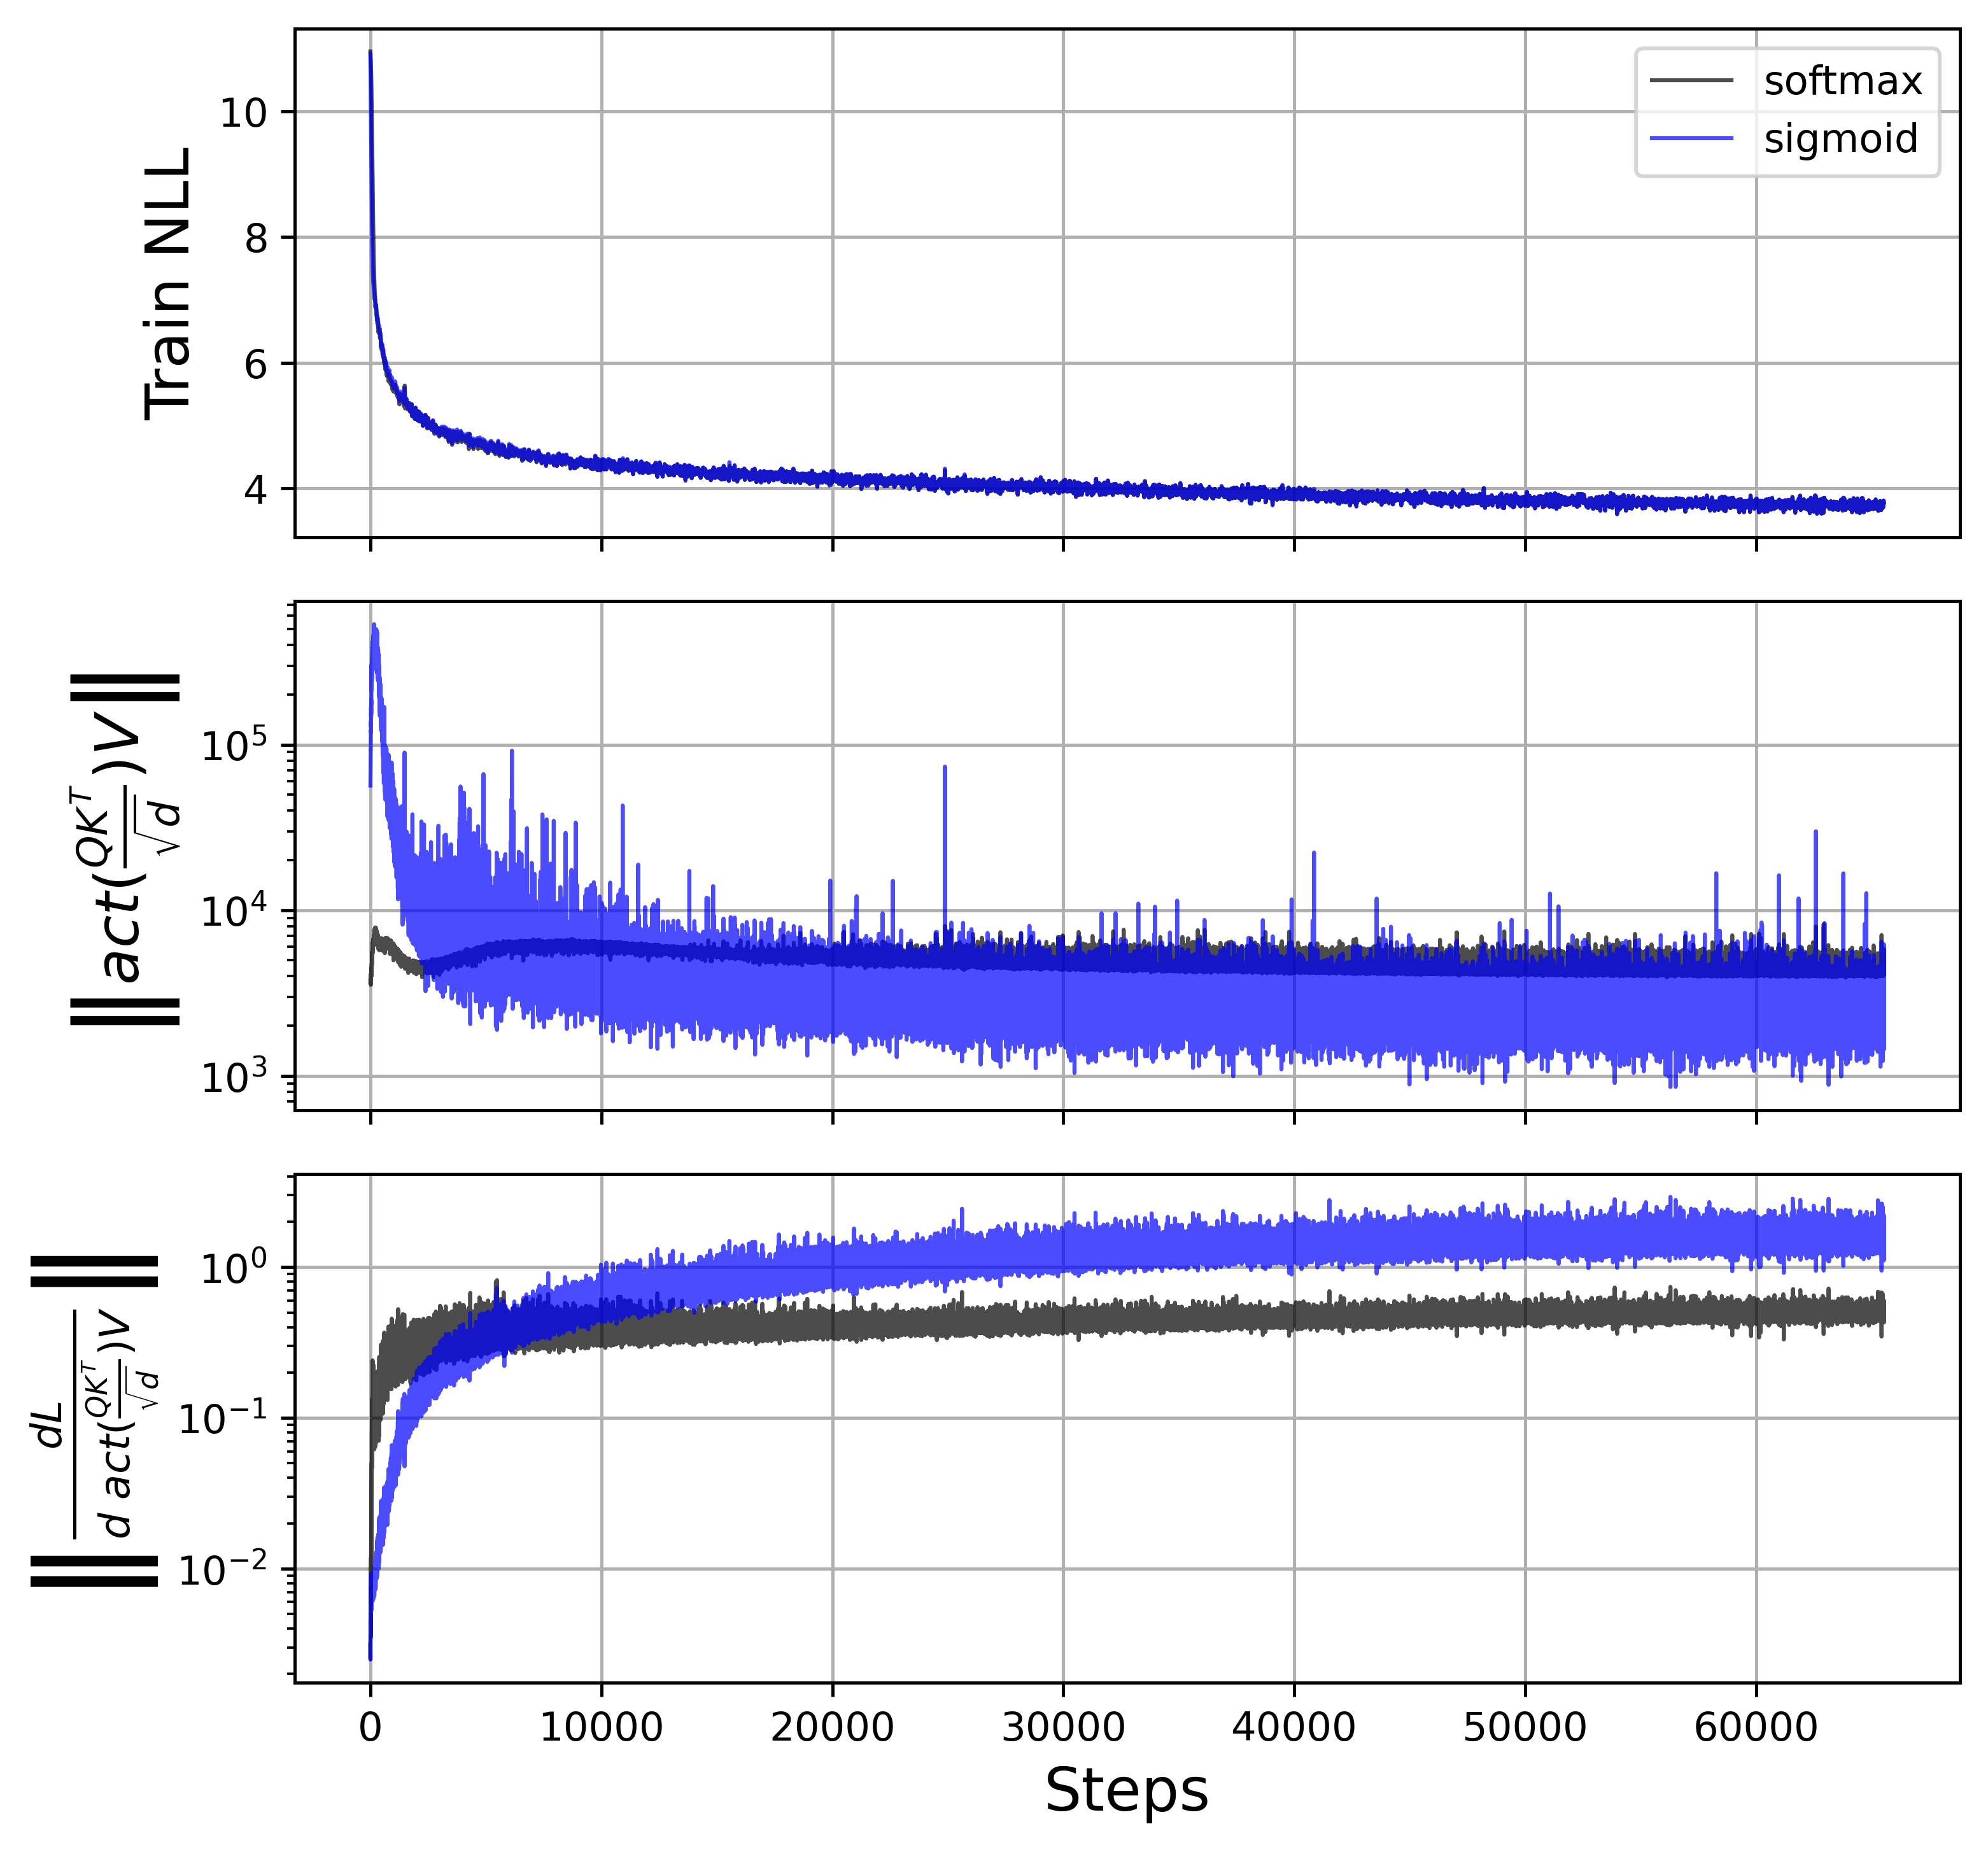
\includegraphics[width=\textwidth]{figures/attn_norm_seed1000001_softmax_vs_sigmoid.png}
        \captionsetup{justification=centering}
        \caption{$b = -\ln n$.}
        \label{fig:no_scaling}
    \end{minipage}\hfill
    \begin{minipage}{0.31\textwidth}
        \centering        
        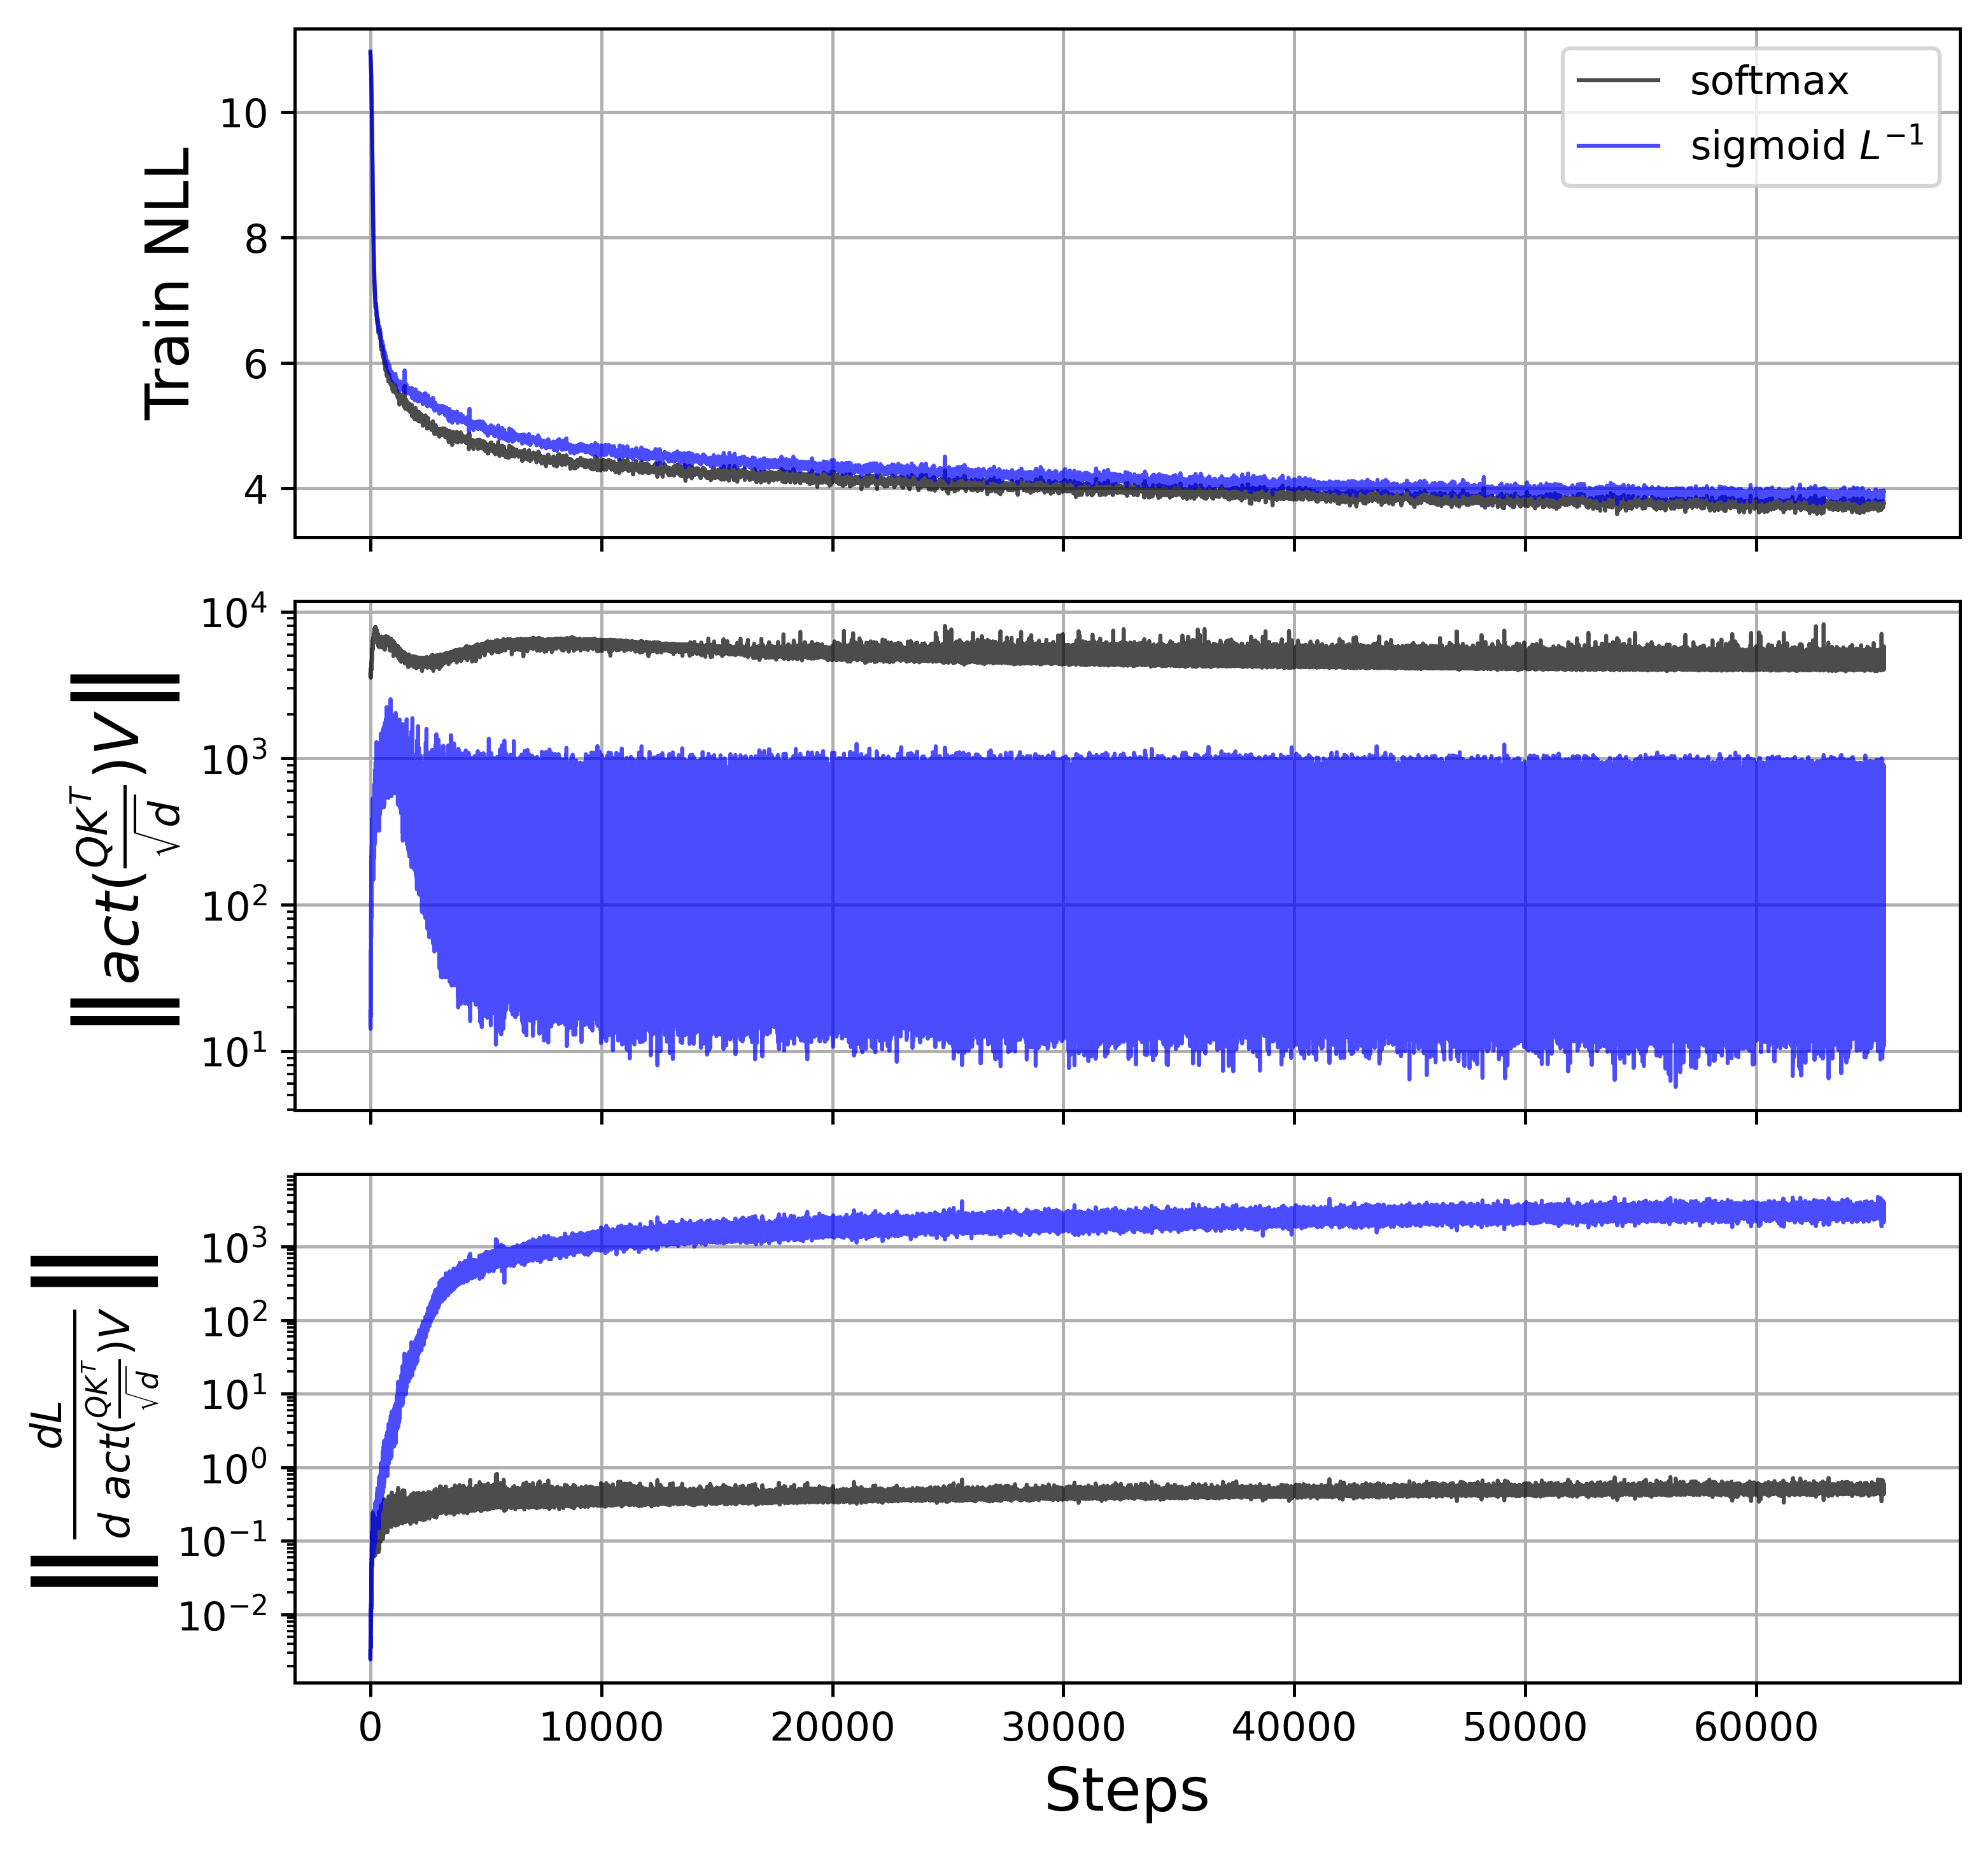
\includegraphics[width=\textwidth]{figures/attn_norm_seed1000001_softmax_vs_sigmoid_seq_len_normalized.png}
        \captionsetup{justification=centering}
        \caption{$n^{-1}$ normalization.}
        \label{fig:seq_len_scaling}
    \end{minipage}\hfill
    \begin{minipage}{0.31\textwidth}
        \centering
        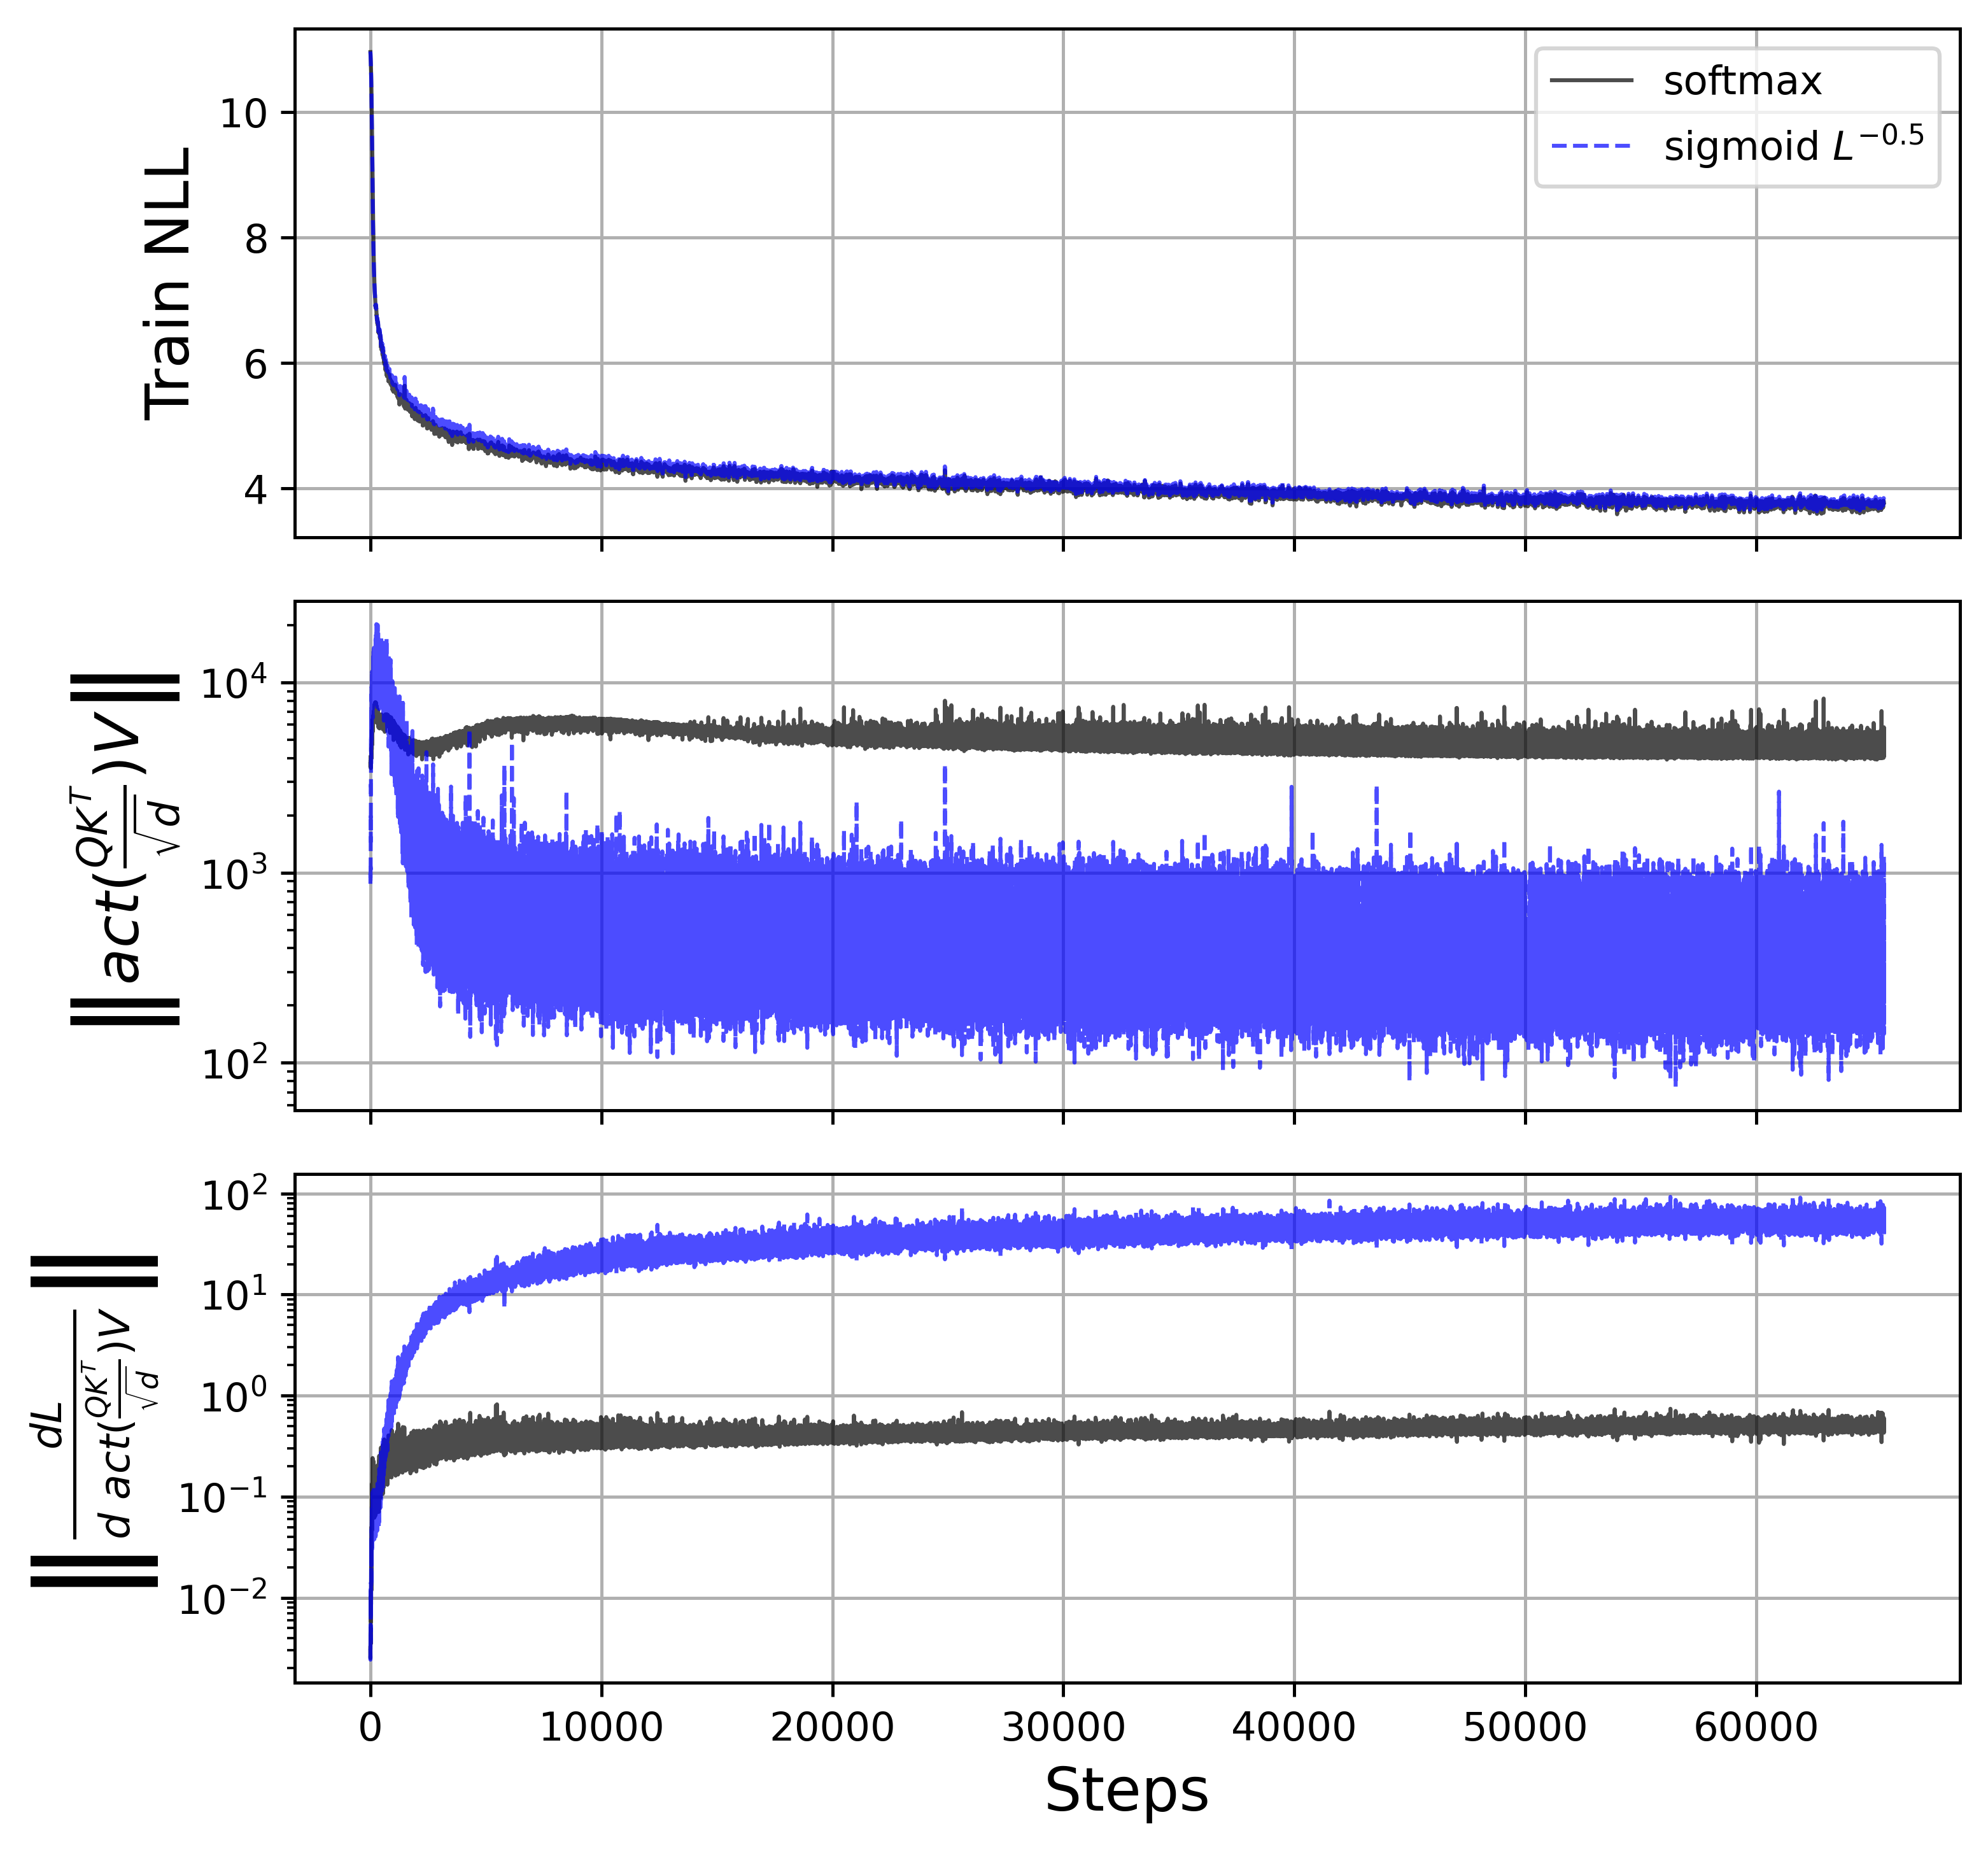
\includegraphics[width=\textwidth]{figures/attn_norm_seed1000001_softmax_vs_sigmoid_sqrt_seq_len_normalized.png}
        \captionsetup{justification=centering}
        \caption{$n^{-0.5}$ normalization.}
        \label{fig:sqrt_scaling}
    \end{minipage}
\end{figure}
\cite{wortsman2023replacing} notes that models trained with sigmoid or ReLU attention require scaling by the sequence length, $n^{-\alpha} \sigma(\mQ\mK^T / \sqrt{d_{qk}})\mV$. We ablate this by comparing the scaled solution to the one we propose in \cref{app:sigmoid_bias}. We also generalize the variant proposed in \citep{wortsman2023replacing} to variadic sequence lengths such that it works with auto-regressive (AR) training, for example for $n=3$:
\begin{align}
    \underbrace{\begin{bmatrix}
        1 & 1 & 1 \\
        0.5^{-\alpha} & 0.5^{-\alpha} & 1 \\
        0.33^{-\alpha} & 0.33^{-\alpha} & 0.33^{-\alpha} \\
    \end{bmatrix}}_{n^{-\alpha}} \odot
    \underbrace{\begin{bmatrix}
        1 & 0 & 0 \\
        1 & 1 & 0 \\
        1 & 1 & 1 \\
    \end{bmatrix}}_{\text{Causal Mask } \mM} \odot \   
     \sigma(\mQ \mK^T / \sqrt{d_{qk}}) \mV .
\label{eqn:ar_seq_len_normalization}
\end{align}
We repeat the experiment from \cref{fig:rope_vs_alibi}, using ALiBi positional embeddings for all trials. We apply $\alpha=\{1, 0.5\}$ AR normalization proposed in \Cref{eqn:ar_seq_len_normalization}. While there is an observable difference in terms of the attention norm, $\lVert \sigma(\mQ \mK^T / \sqrt{d_{qk}}) \mV \rVert$, we find that the train NLL is slightly worse for both normalized variants (\cref{fig:seq_len_scaling,fig:sqrt_scaling}) in comparison to the $b = -\ln n$  variant in \cref{fig:no_scaling}.
\subsubsection{Attention Bias Stability Ablation}
\label{sec:attn_bias_ablation}
To validate the stabilizing effects of attention bias we repeat the experiment from \cref{fig:qk_norm_ablation,fig:layerscale_ablation}, keeping all of the same hyper-parameters, while enabling QK norm and LayerScale (initialized at $10^{-4}$). We train with a range of constant bias offsets, $b \in \{-15, -10, -6, -4, -1 \}$ and visualize the results below in \cref{fig:const_attn_bias_ablation}.
\begin{figure}[htbp]
    \centering
    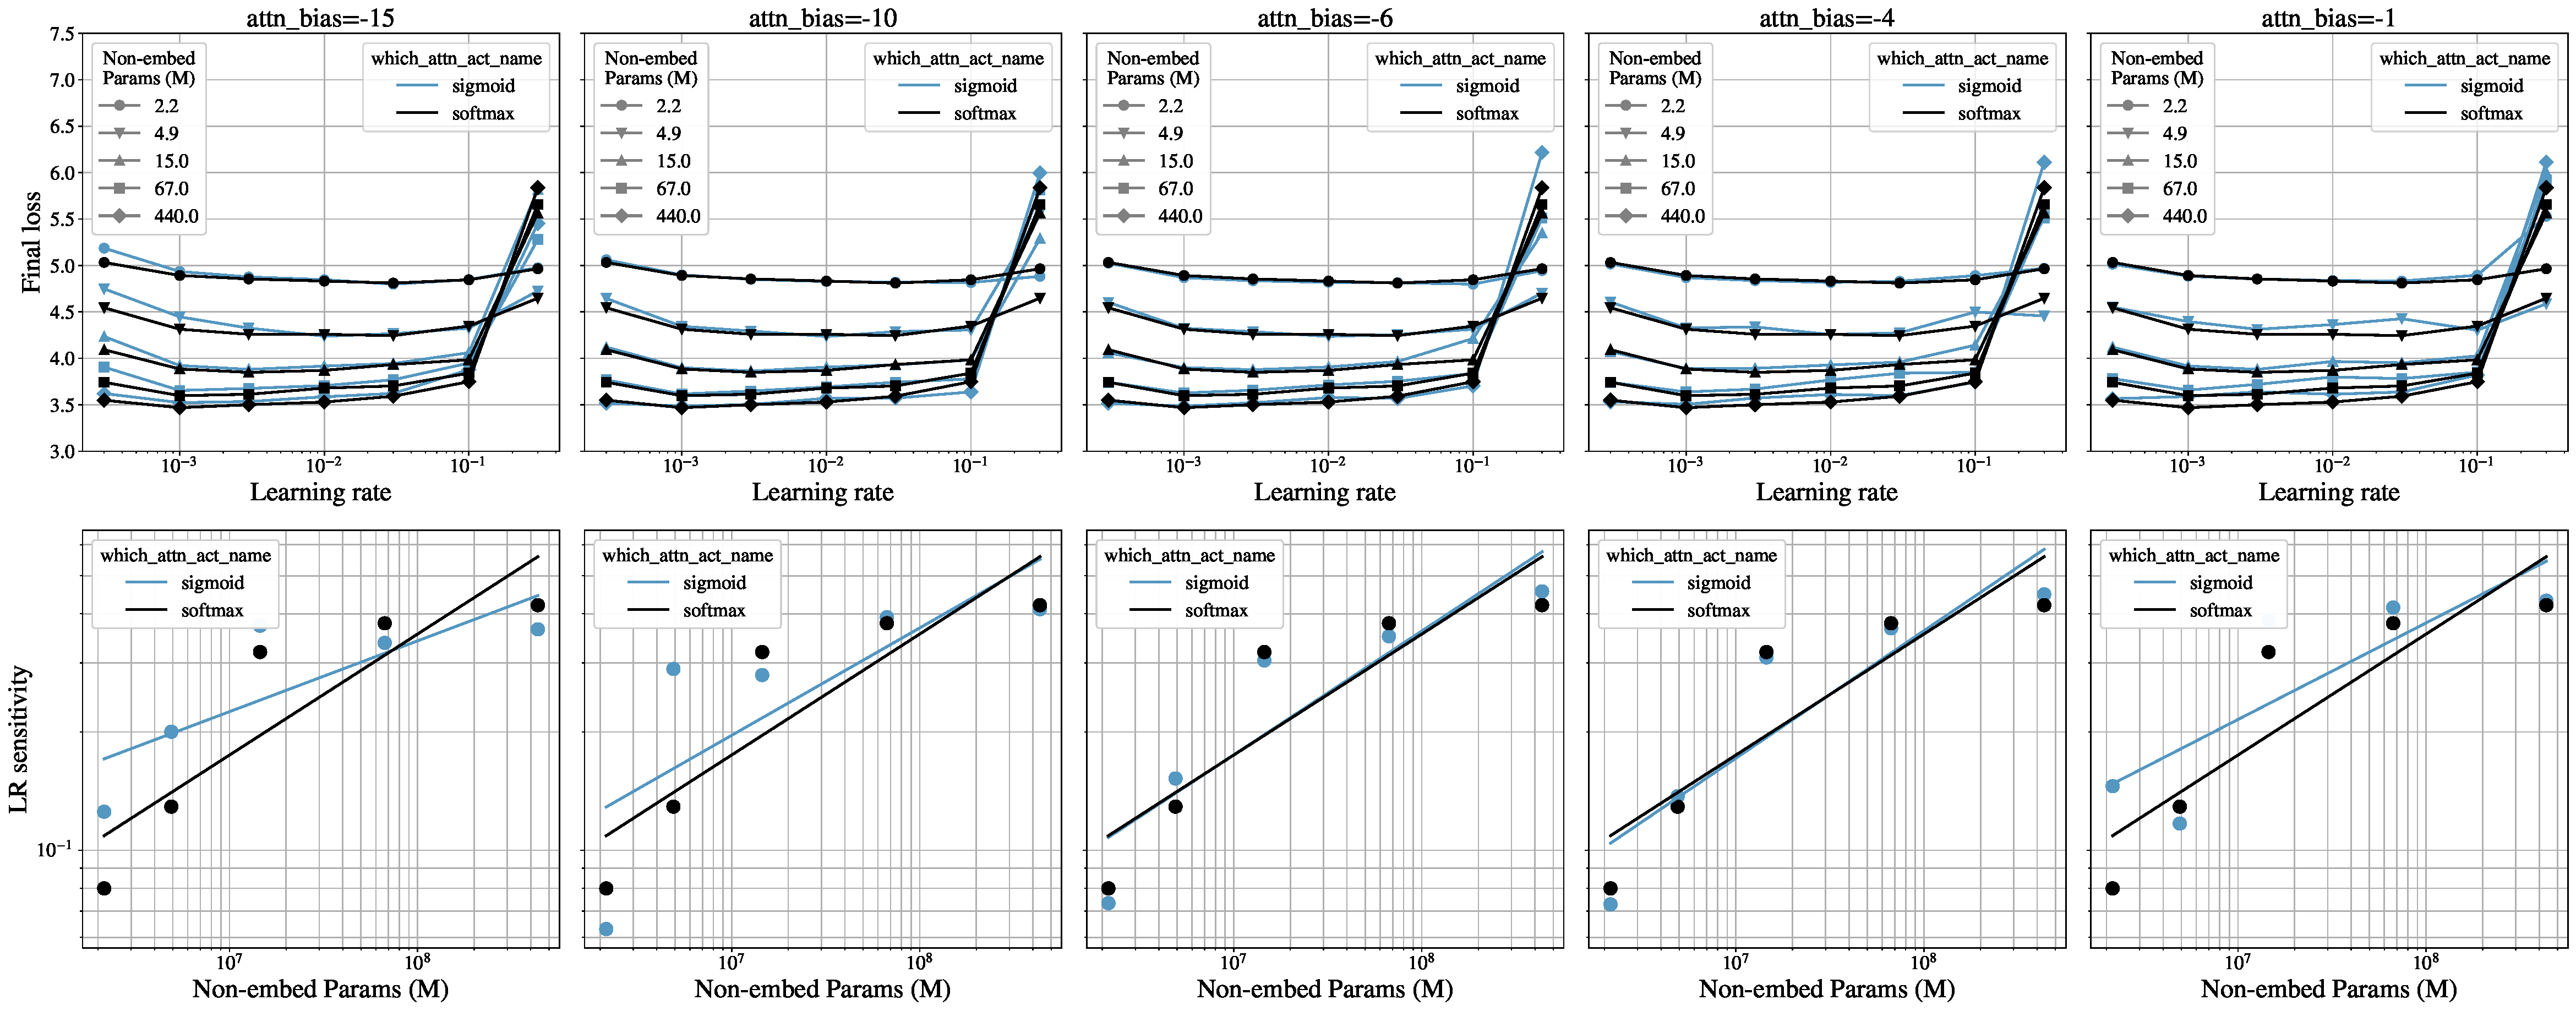
\includegraphics[width=\textwidth]{figures/lines=activation-cols=bias.pdf}
    \captionsetup{justification=centering}
    \caption{Attention bias ablation.}
    \label{fig:const_attn_bias_ablation}
\end{figure}
We observe a systematic increase in stability (and lower $\sigmoidattn$ NLL) for values less than $-1$ up till $-10$, after which the $-15$ plot shows an over-regularizing effect with decreased performance.
\subsection{Vision}
\label{app:vision}
\subsubsection{Test ImageNet1k Top-1\%}
\label{app:top1_results}
\begin{figure}[htbp]
    \centering
    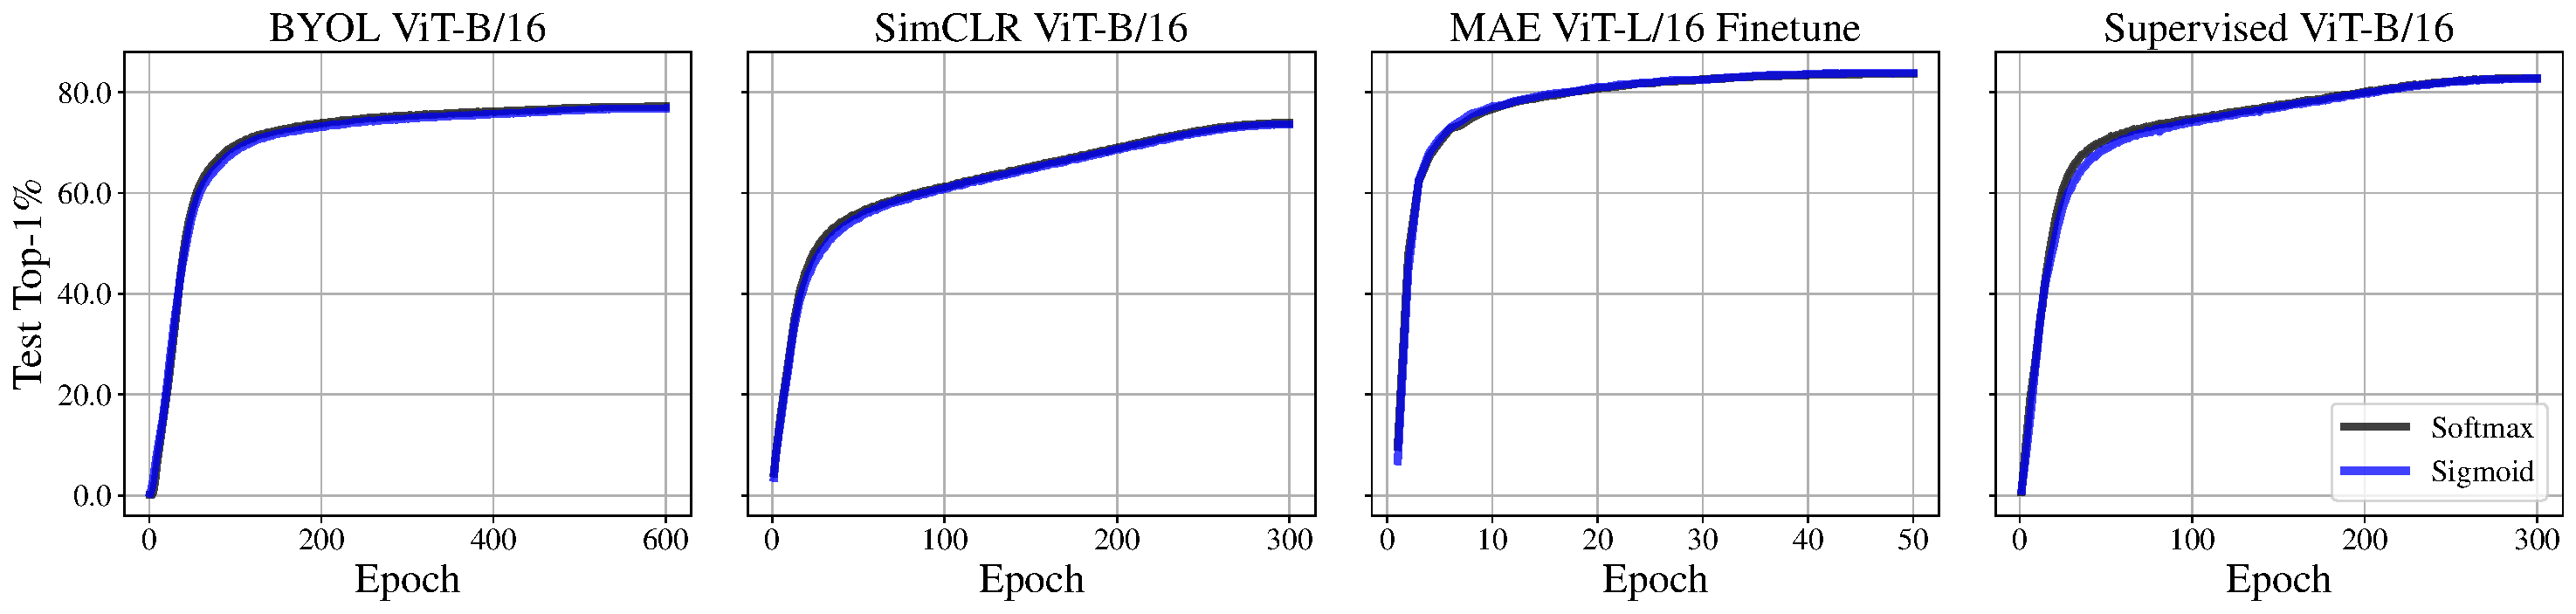
\includegraphics[width=\textwidth]{figures/test_top1_linear_probe_and_MAE_FT.pdf}
    \caption{ImageNet1k test top-1\% for $\softmaxattn$ vs. $\sigmoidattn$ using models from \cref{fig:summary_nll}. %
    }
    \label{fig:test_top1_results}
\end{figure}
\cref{fig:test_top1_results} reports the test linear probe results for the ViT-B/16 BYOL \citep{DBLP:conf/nips/GrillSATRBDPGAP20, DBLP:conf/nips/BusbridgeRALDCW23}, ViT-B/16 SimCLR \citep{DBLP:conf/icml/ChenK0H20, DBLP:conf/icml/ZhaiLLBR0GS23} and the finetuned performance for the ViT-L/16 MAE \citep{DBLP:conf/cvpr/HeCXLDG22} and the test top-1\% results for for ViT-B/16 supervised model \citep{DBLP:conf/iclr/DosovitskiyB0WZ21}.
Across these wide range of SSL and supervised learning tasks, trained with contrastive (SimCLR), EMA distillation (BYOL) and reconstructive objectives (MAE), we find that $\sigmoidattn$ not only matches the training dynamics (\cref{fig:summary_nll}), but also the linear probe and finetuned performance of the baseline $\softmaxattn$.
\subsubsection{LayerScale Free Sigmoid Attention}
\label{sec:layerscale_free_sigmoid}
\begin{figure}[ht]
  \begin{minipage}{0.58\textwidth}
    \centering
    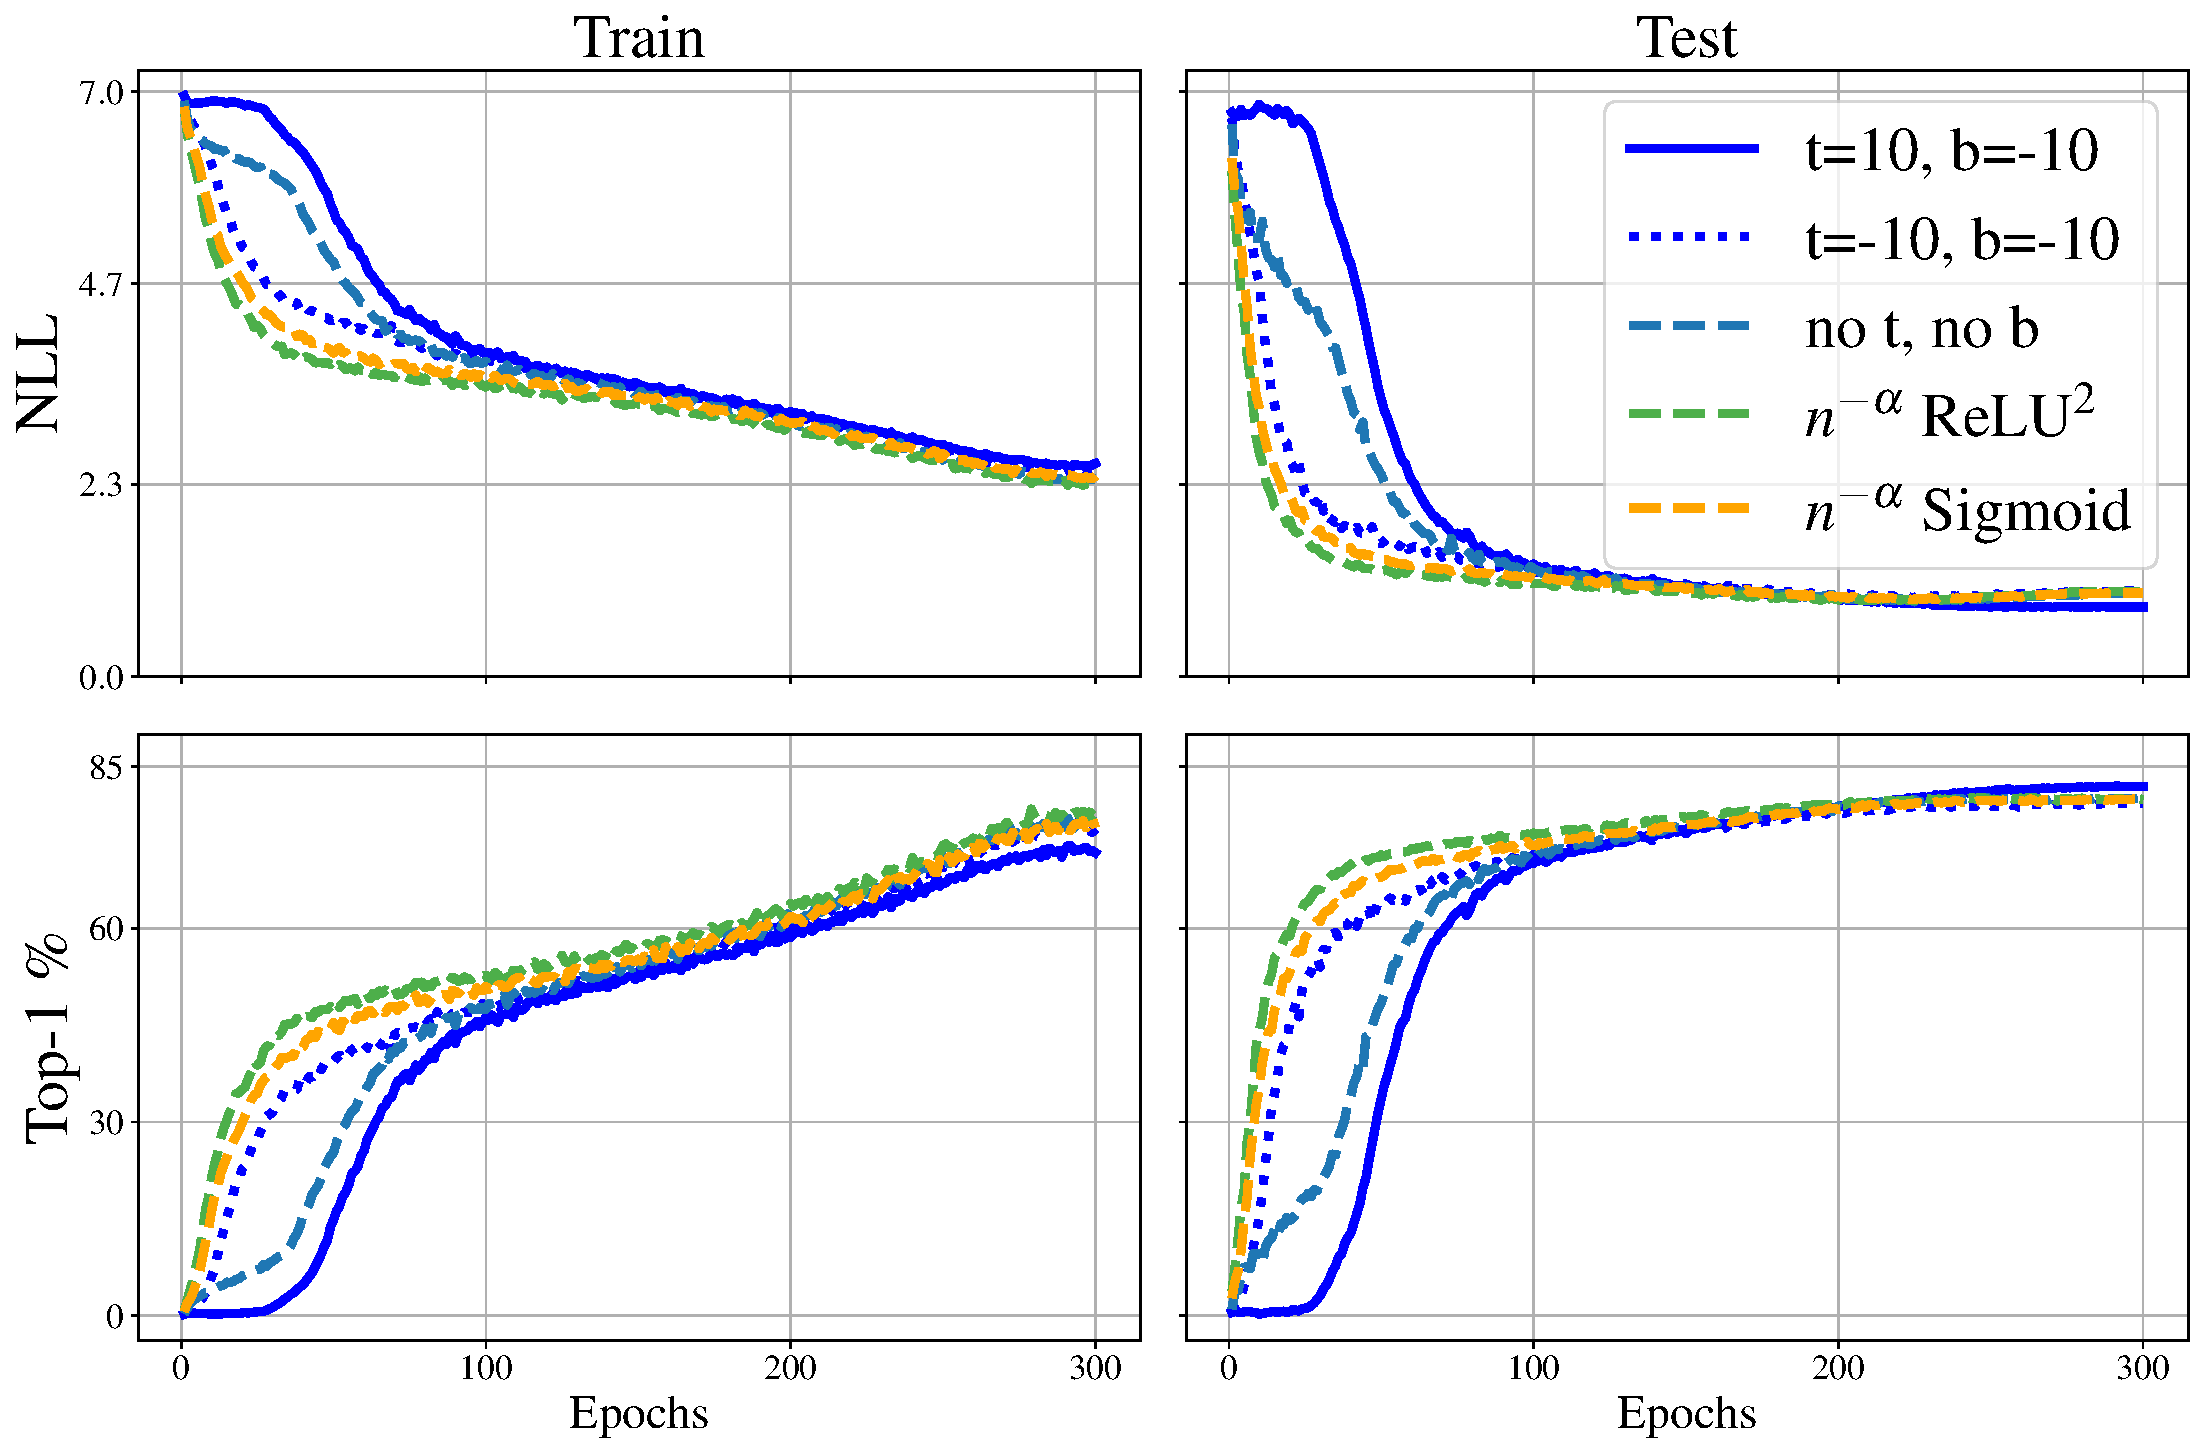
\includegraphics[width=\linewidth]{figures/train_test_metrics_clean.pdf}
  \end{minipage}%
  \hfill
  \begin{minipage}{0.4\textwidth}
    \caption{A competitive $\sigmoidattn$ ViT-B/16 model can be learned without LayerScale or QK norm using a large initial \emph{learnable} scalar temperature $t=10$ and bias $b=-10$ (similar to SigLIP \citep{DBLP:journals/corr/abs-2303-15343}): $\sigma(e^t [\mQ\mK^T / \sqrt{d_{qk}}] + b)\mV, \{b, t\} \in \mathbb{R}$. This regularizes the model, as it must move the temperature to a learnable regime. The $t=10,b=-10$ curve makes no progress in train NLL or test top-1 for $\sim$25 epochs (near max LR), but ultimately outperforms baselines.}    
    \label{fig:layerscale_free_sigmoid}
  \end{minipage}  
\end{figure}
While \cref{fig:layerscale_free_sigmoid} demonstrates the possibility of learning $\sigmoidattn$ without LayerScale, it involves task specific tuning of $\{t, b\}$. We also explored gating attention from learning (through a simple multiply by zero) for $\sim$25 epochs and were able to match the $t = 10, b = -10$ training curves from above. However, we opted for the LayerScale method due to its simplicity.
\subsubsection{Sigmoid Attention vs. Attention Relaxations}
\label{sec:attention_relaxations}
\vspace{-0.1in}
\begin{figure}[ht]
   \begin{minipage}{0.5\textwidth}
    \centering
    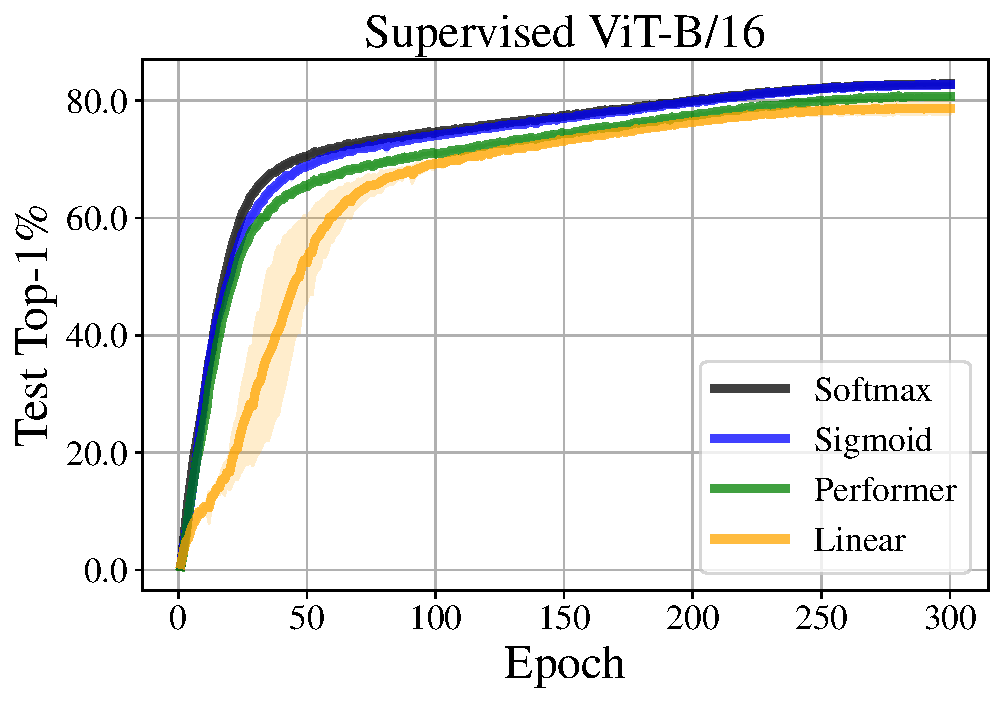
\includegraphics[width=\linewidth]{figures/test_top1_attn_relaxations.pdf}
  \end{minipage}%
  \hfill
  \begin{minipage}{0.48\textwidth}
    \caption{Supervised ViT-B/16 ImageNet1k classification. We contrast $\sigmoidattn$ and $\softmaxattn$ against (a) linear attention with no activation: $\mQ \mK^T / \sqrt{d_{qk}}$ and (b) fast attention via positive orthogonal random features, used in Performer \citep{DBLP:conf/iclr/ChoromanskiLDSG21}. $\sigmoidattn$, like $\softmaxattn$, differs from attention relaxations like Performer which uses low-rank representations of the attention matrix. $\sigmoidattn$ maintains performance parity with $\softmaxattn$, while outperforming other efficient attention variants.}
    \label{fig:attention_relaxations}
  \end{minipage}  
\end{figure}
\subsubsection{Hyper-Parameters}
\label{sec:appendix_vision_hyperparams}
\begin{table}[H]
\centering
\small
\caption{$\sigmoidattn$ SimCLR and BYOL ViT-B/16 hyperparameters.}
\label{tab:sigmoid_simclr_byol_attn_recipe}
\resizebox{0.7\textwidth}{!}{%
\begin{tabular}{lcc}
\toprule
Parameter & SimCLR & BYOL \\
\midrule
Attention bias & None & None \\
LayerScale Init & $10^{-4}$ & $10^{-4}$ \\
QK Norm & Yes & Yes \\
Pos Embed & SinCos & Learnable \\
\midrule
Freeze Patcher & Yes & No \\
Weight init & MocoV3~\citep{DBLP:conf/iccv/ChenXH21} & \texttt{trunc\_normal(.02)} \\
Normalization & LayerNorm & LayerNorm \\
LR schedule & Single Cycle Cosine & Single Cycle Cosine \\
LR warmup & 10 Epochs & 40 Epochs \\
Min LR & $1\times 10^{-6}$ & $1\times 10^{-6}$ \\
Training duration & 300 Epochs & 600 Epochs \\
Optimizer & AdamW & AdamW \\
Optimizer scaling rule & Linear & Linear \\
Base Adam ($\beta_1, \beta_2$) & (0.9, 0.95) & (0.9, 0.95) \\
Base LR & $2\times 10^{-4}$ & $1\times 10^{-4}$ \\
Base batch size & 256 & 256 \\
Total batch size & 4096 & 4096 \\
Base teacher momentum & - & 0.996 \\
Weight decay & 0.1 & 0.3 \\
Weight decay skip bias & Yes & Yes \\
Numerical precision & \texttt{bf16} & \texttt{bf16} \\
Stochastic depth & 0.0 & 0.2 \\
Augmentation stack & SimCLR~\citep{DBLP:conf/icml/ChenK0H20} & DINO multicrop~\citep{DBLP:conf/iccv/CaronTMJMBJ21} \\
Color Jitter Scaling & 0.5~\citep{DBLP:conf/iccv/ChenXH21} & 1.0 \\
\bottomrule
\end{tabular}
}
\end{table}
\begin{table}[H]
\centering
\small
\caption{$\sigmoidattn$ Supervised ViT-B/16 and MAE ViT-L/16 hyperparameters.}
\label{tab:sigmoid_mae_sup_attn_recipe}
\resizebox{0.7\textwidth}{!}{%
\begin{tabular}{lcc}
\toprule
Parameter & Supervised & MAE \\
\midrule
Attention bias & None & $b = - \ln{n}$ \\
LayerScale Init & $10^{-4}$ & $10^{-4}$ \\
QK Norm & Yes & Yes \\
Pos Embed & Learnable & Learnable \\
\midrule
Architecture & ViT-B/16 & ViT-L/16 \\
Mask Ratio & - & 0.75 \\
Freeze Patcher & No & No \\
Weight init & \texttt{trunc\_normal(.02)} & \texttt{trunc\_normal(.02)} \\
Normalization & LayerNorm & LayerNorm \\
LR schedule & Single Cycle Cosine & Single Cycle Cosine \\
LR warmup & 20 Epochs & 40 Epochs \\
Min LR & $1\times 10^{-6}$ & $0.0$ \\
Training duration & 300 Epochs & 400 Epochs \\
Optimizer & AdamW & AdamW \\
Optimizer scaling rule & Linear & Linear \\
Base Adam ($\beta_1, \beta_2$) & (0.9, 0.95) & (0.9, 0.95) \\
Base LR & $1\times 10^{-4}$ & $1.5\times 10^{-4}$ \\
Base batch size & 256 & 256 \\
Total batch size & 4096 & 4096 \\
Weight decay & 0.3 & 0.05 \\
Weight decay skip bias & Yes & Yes \\
Numerical precision & \texttt{bf16} & \texttt{bf16} \\
Stochastic depth & 0.28 & 0.0 \\
Augmentation stack & RandAug~\citep{DBLP:conf/nips/CubukZS020} & RRC + HFLIP \\
\bottomrule
\end{tabular}
}
\end{table}

\subsection{Language Model}
\label{sec:llm_appendix}
\subsubsection{Hyper-Parameters}
\begin{table}[h]
\centering
\caption{Training details for the Llama-style 1B LM training.}
\label{tab:lm_training_details}
\resizebox{0.35\textwidth}{!}{%
\begin{tabular}{@{}lll@{}}
\toprule
 & Parameter          & Value     \\ \midrule
 & Params             & 1B        \\
 & Context Length     & 2048      \\
 & Total Tokens       & 300B        \\
 & Batch size         & 4M tokens \\
 & LR Schedule        & Cosine    \\
 & LR Warmup Steps    & 5000      \\
 & Peak LR            & 1e-2      \\
 & Final LR           & 10\% of peak \\
 & Optimizer          & AdamW     \\
 & Optimizer momentum & 0.9, 0.95 \\
 & Weight decay       & 1e-4       \\
 & Gradient clipping  & 1.0       \\
 & Position encoding  & ALiBi     \\
 & Q/K Norm           & Applied   \\
 & Num layers         & 24        \\
 & Num heads          & 32        \\
 & Hidden dim         & 2048      \\
 &                    &           \\ \bottomrule
\end{tabular}
}
\end{table}
\cref{tab:lm_training_details} shows the hyper-parameters for the final comparison. MuP-simple \citep{DBLP:journals/corr/abs-2309-14322} is used, where the peak learning rate is set to 1e-2. Weight decay is decoupled, following \cite{loshchilov2017decoupled}. In addition, to confirm that applying QK-Norm does not hurt the baseline, we show training parity with and without QK-Norm in \cref{fig:lm_1b_qknorm}.
\begin{figure}[h]
    \centering
    \begin{minipage}{0.46\textwidth}
        \footnotesize
        \centering
        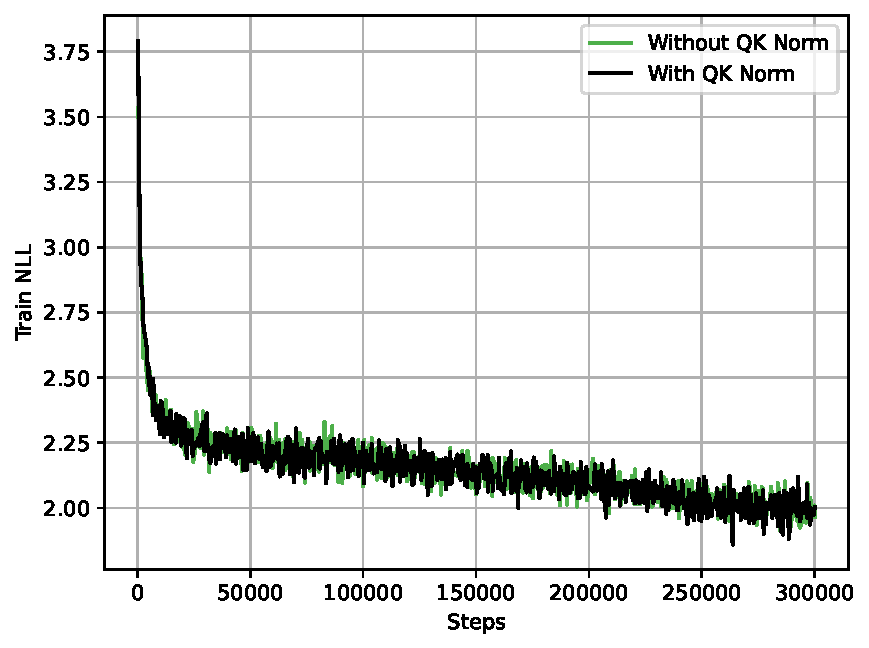
\includegraphics[trim={0 0 0 0}, width=\textwidth]{
            figures/llm/1b_qknorm.pdf
        }
        \captionsetup{justification=centering}
        \caption{
            1B $\softmaxattn$ LLM training with and without QK Norm, converging to the same loss.
        }
        \label{fig:lm_1b_qknorm}
    \end{minipage}
    \hfill
    \begin{minipage}{0.46\textwidth}
        \centering        
        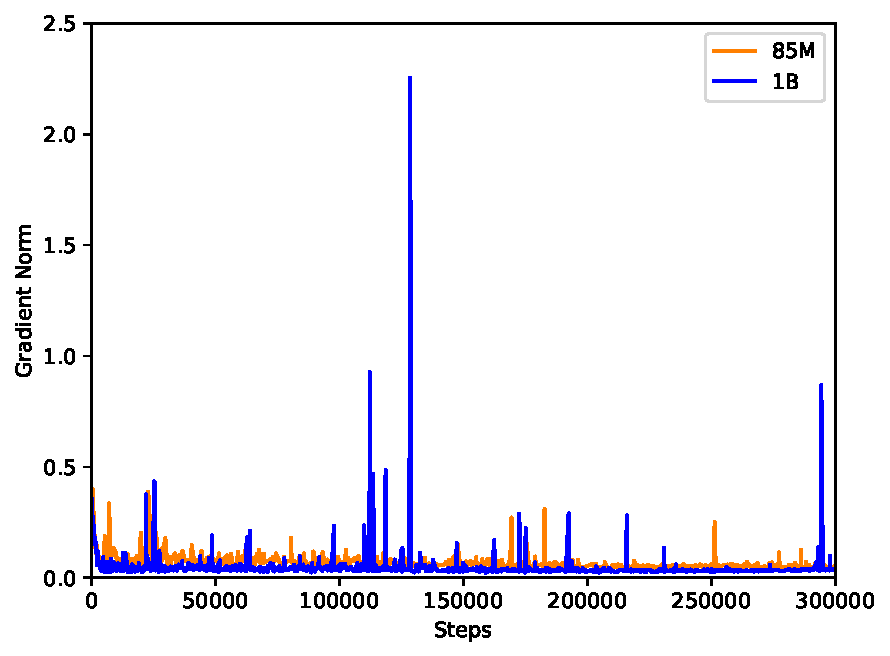
\includegraphics[trim={0 0 0 0}, width=\textwidth]{
            figures/llm/grad_norm.pdf
        }
        \captionsetup{justification=centering} 
        \caption{85M and 1B LLM training using $\sigmoidattn$ (n = 4096). Smooth training loss curves, but gradient norm shows spikes.}
        \label{fig:lm_grad_norm}
    \end{minipage}
\end{figure}
\begin{figure}[H]
    \centering
    \begin{minipage}{0.46\textwidth}
        \footnotesize
        \centering
        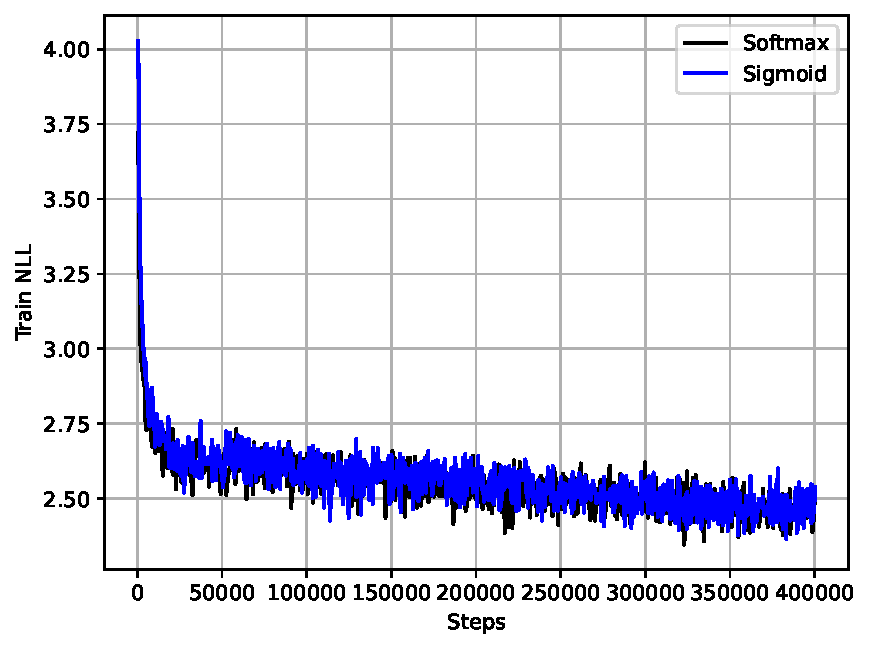
\includegraphics[trim={0 0 0 0}, width=\textwidth]{
            figures/llm/85m_nll.pdf
        }
        \captionsetup{justification=centering}
        \caption{
            85M training using $\sigmoidattn$ and $\softmaxattn$ (n = 4096). Training loss matches.
        }
        \label{fig:85m_4k_nll}
    \end{minipage}
    \hfill
    \begin{minipage}{0.46\textwidth}
        \centering        
        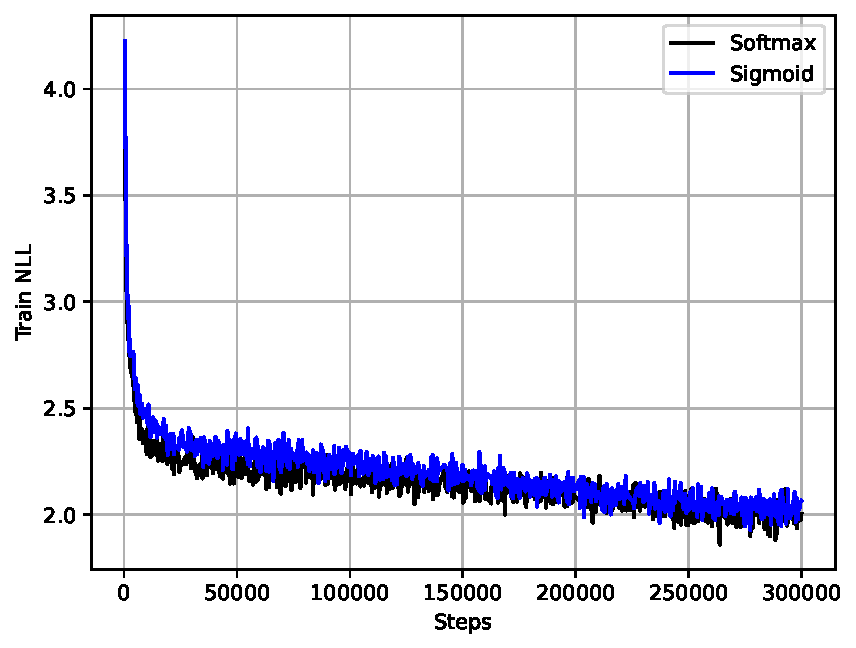
\includegraphics[trim={0 0 0 0}, width=\textwidth]{
            figures/llm/1b_nll.pdf
        }
        \captionsetup{justification=centering} 
        \caption{1B training using $\sigmoidattn$ (n = 4096). Higher sequence length with a larger model shows a slightly different loss curve.}
        \label{fig:1b_4k_nll}
    \end{minipage}
\end{figure}
\subsubsection{Gradient Norm}
While a $\sigmoidattn$ based LM using aforementation hyper-parameters has a smooth loss curve, we do see more gradient norm fluctuations. See \cref{fig:lm_grad_norm}, where spikes larger than $0.5$ are not visible in the $\softmaxattn$ equivalent.

\subsection{Automatic Speech Recognition}
\label{sec:asr_hps}

\subsubsection{Training Details}
All acoustic models are fed 80 channel log-mel filterbanks with a 25ms sliding window strided by 10ms. 

The transformer-based encoder model has 255M parameters: 1D convolution of kernel 7 and stride 3 followed by CAPE positional embedding if it is used and 36 transformer blocks with pre-LayerNorm, an embedding dimension of 768, 4 heads, 3072 units in the MLP layers.
The model is trained with CTC loss and a character vocabulary, including apostrophe (`). 
In additional experiments, we vary the depth to 12 and 24 layers, and change pre-LayerNorm to post-LayerNorm.

We implemented our own conformer-based encoder model, also trained  with a CTC loss and a character vocabulary.
The conformer model has 104M parameters and consists of 1D convolution of kernel 7 and stride 3 followed by 16 conformer blocks with an embedding dimension of 512, 4 heads, 2048 units in the MLP layers. 
Variational noise is not used and RoPE is used as a relative positional embedding instead of relative sinusoidal positional embedding.

For all models, SpecAugment~\citep{DBLP:conf/interspeech/ParkCZCZCL19} is used for augmentation with 2 frequency masks (max width 30) and 10 time masks (max width 50, ratio 0.1). 
All models are trained with dynamic batching and mixed precision with BF16.
Models are trained with different configurations of optimizers and hyperparameters to have diverse coverage of use-cases. 
\textbf{\textit{We first optimize every configuration for $\softmaxattn$ and then change only attention to the introduced configuration of $\sigmoidattn$ while all other parameters are kept the same.}}
Detailed configurations are shown in~\Cref{tab:asr-training-details}.
We train models until the greedy WER stops improving on the validation sets (\textit{dev-clean, dev-other}) and report final test sets (\textit{test-clean, test-other}) greedy WER without integration of any external language model.

For the bias term $b=-\log n$ in $\sigmoidattn$, we do not use max sequence length as in language model experiments. Instead, for every audio sample we use its own duration as a bias terms resulting into non-trainable bias vector for the minibatch. For experiments with sequence normalization, we also use not the max sequence length in the minibatch but rather the ground truth sample duration to properly normalize encoder attention.


\begin{table}[t!]
\centering
\caption{Training details for the ASR models on LibriSpeech 100h (LS-100) and LibriSpeech 960h (LS-960) for transformers and conformers.}
\label{tab:asr-training-details}
\resizebox{\textwidth}{!}{
\begin{tabular}{@{}llllll@{}}
\toprule
 & Parameter          & Transformer LS-960 & Conformer LS-960 & Transformer LS-100 & Transformer LS-100     \\ \midrule
 & Params             & 255M & 104M & 255M / 170M / 85M        & 255M \\
 & LayerNorm & pre & pre + post & pre & post \\
 & Dropout & 0.1 & 0.1 & 0.3 & 0.3 \\
 & Layer drop & 0.1 & 0.0 & 0.3 & 0.3 \\
 & Training steps      & 400k & 400k & 400k & 500k \\
 & Batch size         & 3.56h & 4.44h & 1.1h & 1.1h \\
 & LR schedule        & step-wise & step-wise & step-wise &  step-wise   \\
 & SpecAugment start & 0k & 10k & 0k & 0k \\
 & LR Warmup Steps    & 64k & 10k & 64k & 64k     \\
 & Peak LR            &  1e-3 & 2e-3 & 0.1 & 0.03   \\
 & LR start decay    & 250k & 250k & 200k & 330k     \\
 & LR decay step  & 50k & 50k & 30k & 50k     \\
 & Optimizer          & AdamW & AdamW & Adagrad & Adagrad    \\
 & Optimizer momentum & 0.9, 0.999 & 0.9, 0.98 & - & - \\
 & Weight decay       & 1e-6 & 1e-6 &   0 & 0     \\
 & Gradient clipping  & 1.0 & 0.5 & 1.0  & 1.0     \\
 & Position encoding  & CAPE / ALiBi / RoPE & RoPE & CAPE & CAPE / ALiBi / RoPE     \\
 & Q/K Norm $\softmaxattn$          & Not Applied & Not Applied &  Not Applied & Not Applied  \\
 & Q/K Norm $\sigmoidattn$          & Applied & Applied &  Not Applied & Applied  \\
 & Num layers         & 36 & 16 & 36 / 24 / 12  & 36      \\
 & Num heads          & 4 & 4 & 4 & 4        \\
 \bottomrule
\end{tabular}
}
\end{table}

To evaluate behaviour for length generalization we use TED-LIUM v3 dataset~\citet{hernandez2018ted} as its validation and test sets have longer audio duration than LibriSpeech: LibriSpeech has in average 10-15s duration, while in TED-LIUM there are audio longer than 30s (the max duration of LibriSpeech).
To perform evaluation on TED-LIUM v3, we combine together validation and test sets of TED-LIUM v3 (we don't use them for training and hyper-parameters search and just perform final evaluation) and split them into 4 datasets according to the duration: 0-10s, 10-20s, 20-30s, and 30s+.

For positional embeddings we use not only CAPE, but change it to AliBi or RoPE. 
As ALiBi was originally introduced for the decoder only models and there is no official adoption of it yet\footnote{See discussion in \url{https://github.com/ofirpress/attention_with_linear_biases/issues/5}.} for the encoder models (without causal masking), we follow the best practices found in \url{https://iclr-blogposts.github.io/2024/blog/alibi-mlm/} of nonsymmetric ALiBi with different slopes instead of symmetric version used by~\citep{lee2022littlebird}.

\begin{table}[t!]
\centering
\caption{Word error rate (\%) on LibriSpeech dev/test sets and TED-LIUM v3~\citep{hernandez2018ted} (``TED'', joint validation and test sets with split according to audio duration) for pre-LayerNorm transformer (255M~/ 170M / 85M params) with CAPE and with either $\softmaxattn$ or $\sigmoidattn$ (w/ LayerScale, w/o QK norm, w/ $b=-\log n$) trained on LibriSpeech 100h data (average duration is 10-15s). Hyper-parameters can be found in \Cref{tab:asr-training-details}.}
\label{tab:asr-pre-100h}
\begin{center}
\begin{scriptsize}
\begin{sc}
\resizebox{\columnwidth}{!}{
\begin{tabular}{lc|rrrr|rrrr}
\toprule
 attn & \# layers & dev-clean & test-clean & dev-other & test-other & ted 0-10s & ted 10-20s & ted 20-30s & ted 30s+  \\
\midrule 
softmax &  36 & 6.7 & 7.1 & 20.0 & 20.4 & 26.4 & 22.4 & 23.3 & 21.8 \\
sigmoid & 36 & 7.0 & 7.3 & 20.3 & 20.5 & 26.2 & 23.4 & 23.6 & 21.8 \\
\,\,\,\, $b=0$  & 36 & 6.8	& 7.1	& 19.8	& 20.3
\\
\midrule
softmax &  24 & 6.4 & 6.8 & 20.2 & 20.5 & 25.4 & 22.1 & 23.3 & 21.8 \\
sigmoid &  24 & 7.1 & 7.3 & 21.0 & 21.3 &  26.6 & 23.3 & 24.0 & 22.0 \\
\,\,\,\, $b=0$ & 24 & 6.7	& 6.9	& 20.2	& 20.7
 \\
\midrule
softmax &  12 & 8.2 & 8.7 & 25.0 & 25.4 & 29.0 & 25.6 & 27.1 & 27.4 \\
sigmoid & 12 & 8.3 & 8.7 & 24.8 & 25.2 & 29.0 & 25.7 & 26.3 & 25.5 \\
\,\,\,\, $b=0$ & 12 & 8.7	& 8.5	& 24.4	& 24.7
\\
\bottomrule
\end{tabular}
}
\end{sc}
\end{scriptsize}
\end{center}
\end{table}


\begin{table}[t!]
\centering
\caption{Word error rate (\%) on LibriSpeech dev/test sets for post-LayerNorm transformer (255M) with either $\softmaxattn$ (w/o QK norm) or $\sigmoidattn$ (by default w/ LayerScale, w/ QK norm, w/ $b=-\log n$) trained on LibriSpeech 100h data. Hyper-parameters can be found in \Cref{tab:asr-training-details}.}
\label{tab:asr-post-100h}
\begin{center}
\begin{scriptsize}
\begin{sc}
\begin{tabular}{lc|rrrr}
\toprule
 attn & PE & dev-clean & test-clean & dev-other & test-other \\
\midrule 
softmax & CAPE & 6.4 & 6.5 & 18.4 & 18.2 \\
\,\,\,\, + QK norm & & 6.1 & 6.3 & 18.2 & 18.1  \\
sigmoid & & 8.0 & 8.4 & 22.7 &  22.7\\
\,\,\,\, - QK norm & & 7.5 & 7.9 & 22.1 & 27.6 \\
\,\,\,\, - LayerScale & & \multicolumn{4}{c}{unstable, gradient norm and loss spikes} \\
\,\,\,\, - QK norm - LayerScale & & 6.5 & 6.9 & 19.9 & 20.1 \\ 
sigmoid ($b=-10$, learnable)  & & 8.7 & 9.4 & 23.5 & 24.0 \\
\midrule
softmax & RoPE & 6.6 & 6.9 & 18.3 & 18.5 \\
sigmoid & & 6.8 & 7.1 & 20.8 & 20.8\\
sigmoid ($b=-10$, learnable)  & & 8.7 & 9.4 & 23.5 & 24.0 \\
\midrule
softmax & AliBi & 6.4 & 6.9 & 18.3 & 18.3 \\
sigmoid & & 6.9 & 7.2 & 20.8 & 21.1 \\
sigmoid ($b=-10$, learnable)  & & 6.8 & 7.1 & 20.4 & 20.5\\
\bottomrule
\end{tabular}
\end{sc}
\end{scriptsize}
\end{center}
\end{table}


\begin{table}[t!]
\centering
\caption{Word error rate (\%) on LibriSpeech dev/test sets and TED-LIUM v3~\citep{hernandez2018ted} (``TED'', joint validation and test sets with split according to audio duration) for conformer (104M) with RoPE and with either $\softmaxattn$ or $\sigmoidattn$ (w/ LayerScale, w/ QK norm, w/ $b=-\log n$) trained on LibriSpeech 960h data (average duration is 10-15s). Hyper-parameters can be found in \Cref{tab:asr-training-details}.}
\label{tab:asr-conformer}
\begin{center}
\begin{scriptsize}
\begin{sc}
\resizebox{\columnwidth}{!}{
\begin{tabular}{l|rrrr|rrrr}
\toprule
 attn & dev-clean & test-clean & dev-other & test-other & ted 0-10s & ted 10-20s & ted 20-30s & ted 30s+  \\
\midrule 
softmax & 2.2	&2.5	& 5.4	&5.6	&13.0 & 11.1	&13.2	&7.1 \\
sigmoid  & 2.3	&2.5	&5.6	&5.8	&13.5	&10.8	&13.3	&10.2 \\
sigmoid ($b=-10$, learnable)  &  2.4&	2.7&	5.8&	5.8&	12.9&	11.1&	14.1&	54.9  \\
\bottomrule
\end{tabular}
}
\end{sc}
\end{scriptsize}
\end{center}
\end{table}

\begin{figure}[t]
    \centering
    
        \centering
        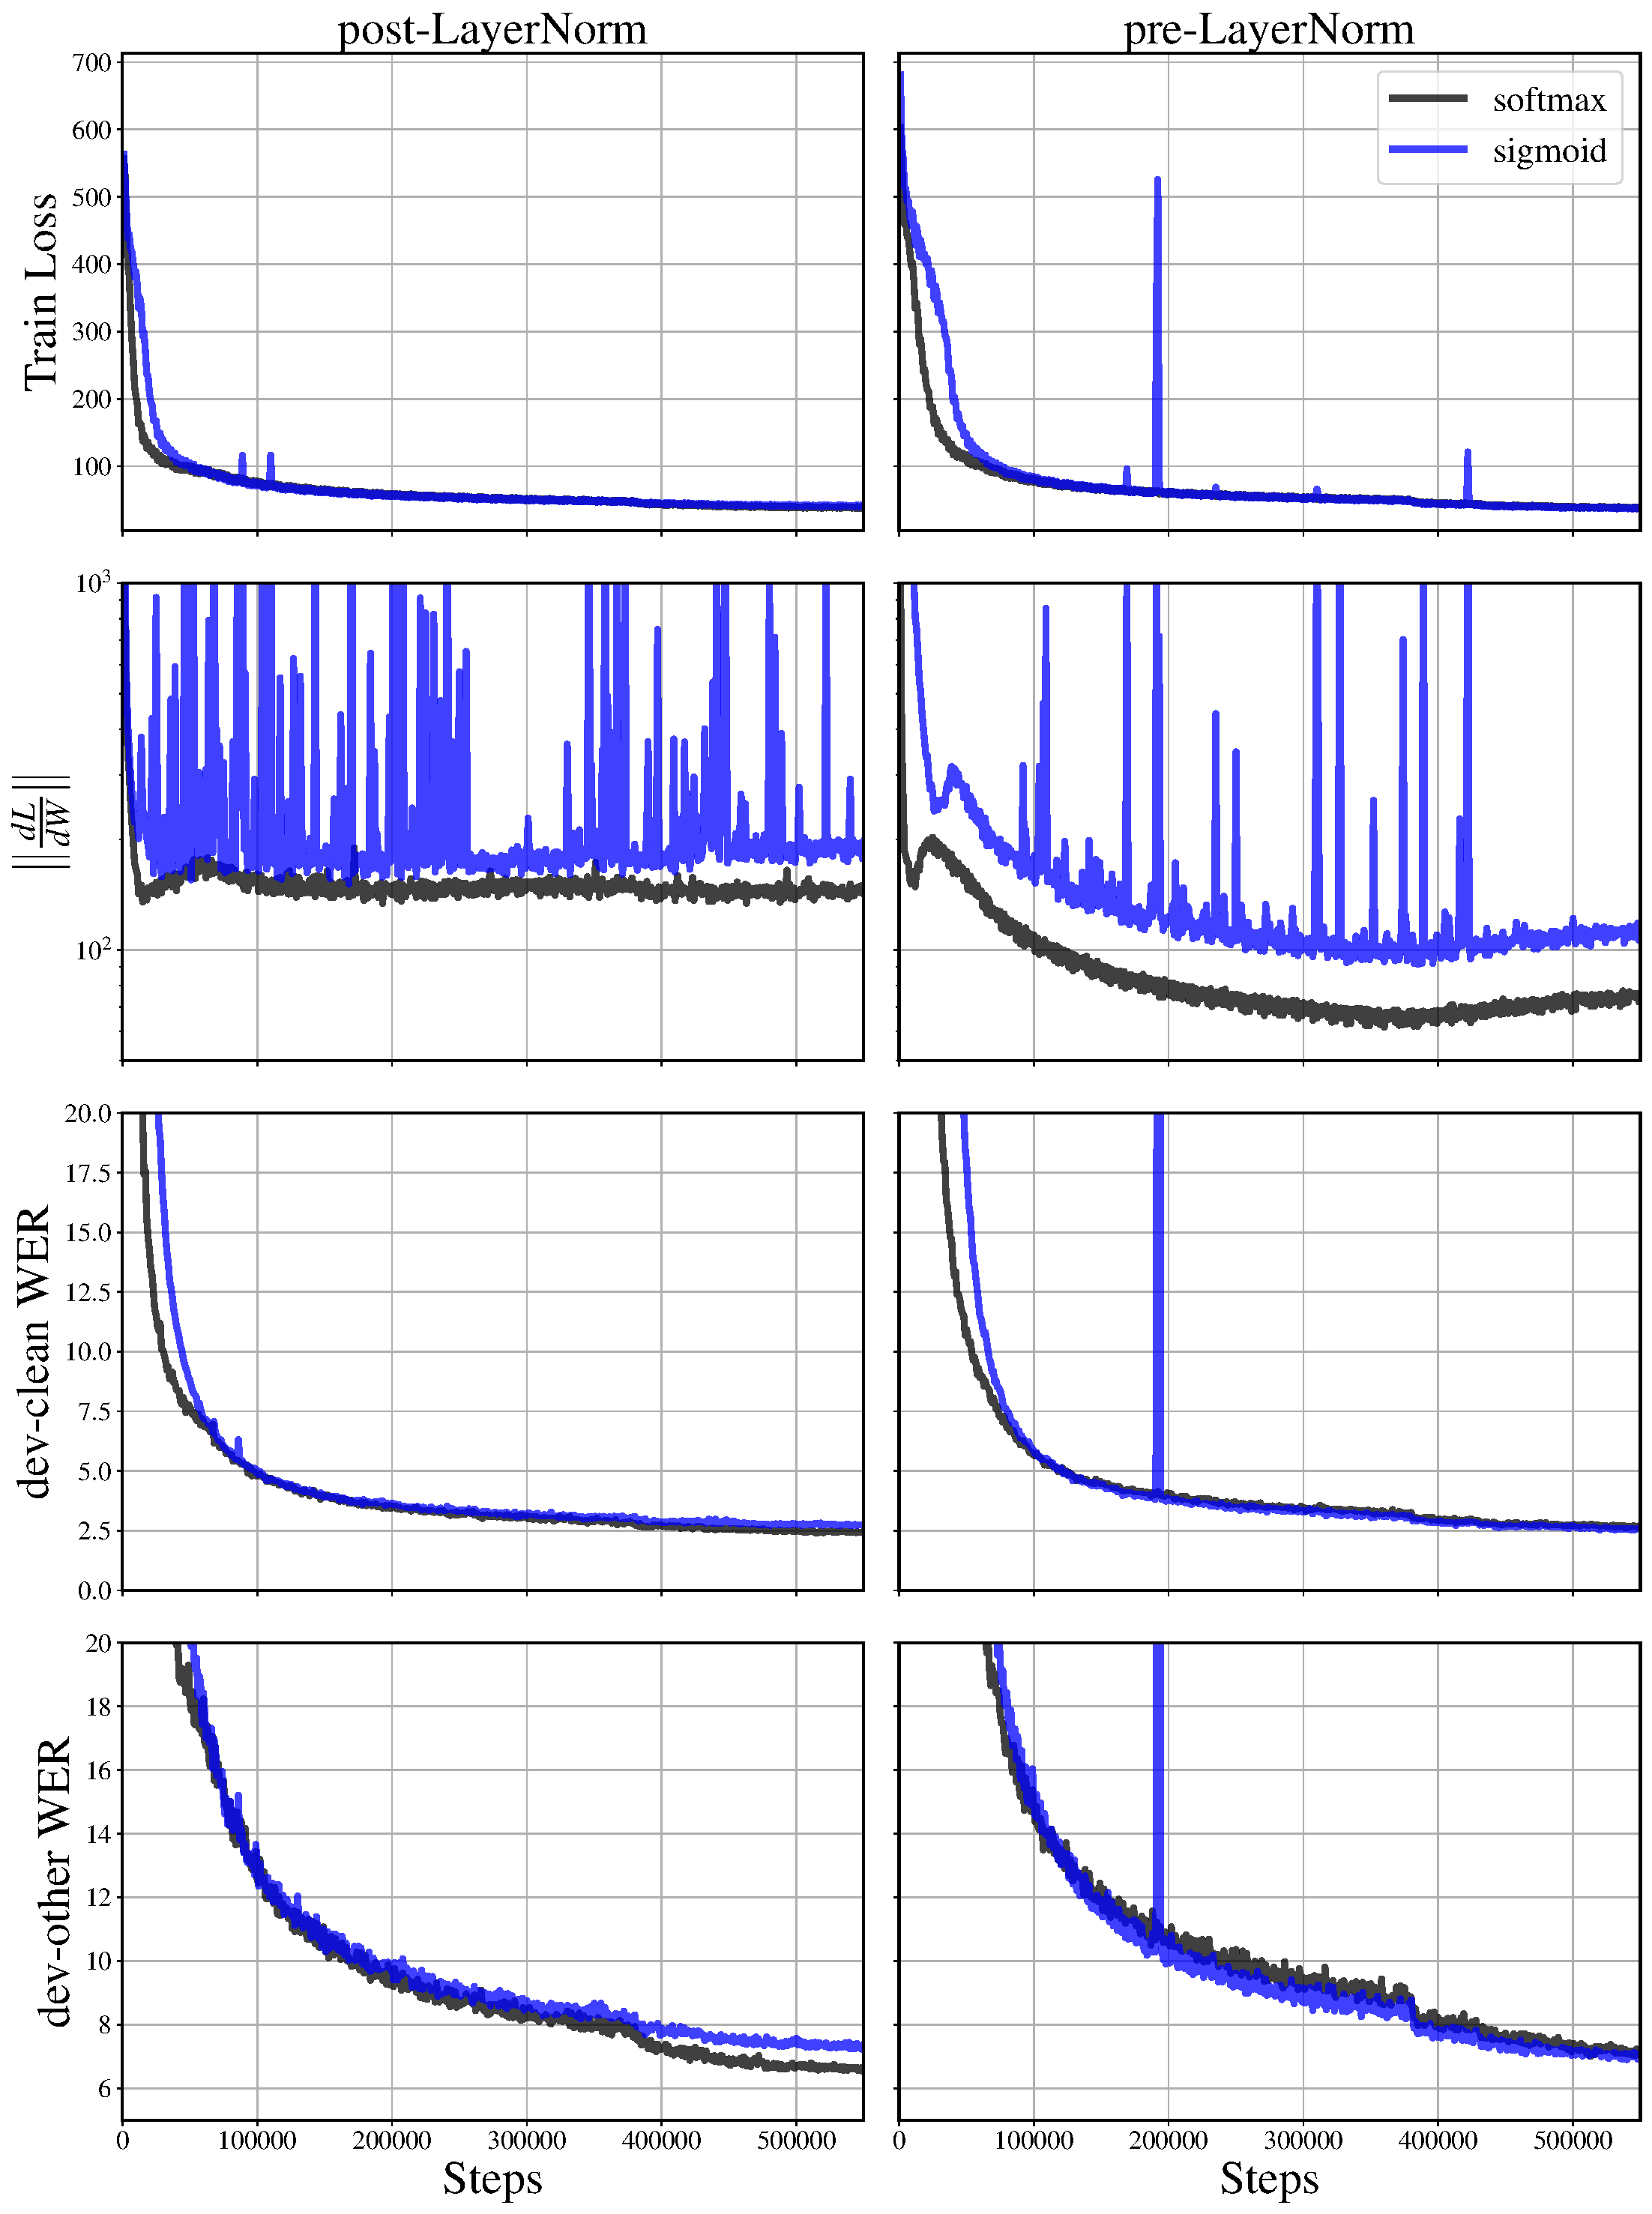
\includegraphics[width=0.6\textwidth]{
            figures/asr_appendix
        }
        \caption{
            ASR Transformer model (255M) training with post-LayerNorm (left) and pre-LayerNorm (right) on LibriSpeech 960h with $\sigmoidattn$ (w/ bias term, $b=0$, w/o QK norm, w/ LayerScale) or with $\softmaxattn$. Huge gradient norms and training loss spikes are observed for $\sigmoidattn$ which can result in worse final model performance hence models for $\sigmoidattn$ are unstable.}
        \label{fig:asr-spikes}
        \vspace{-0.4cm}
\end{figure}

\begin{figure}[ht]
  \begin{minipage}{0.58\textwidth}
    \centering
    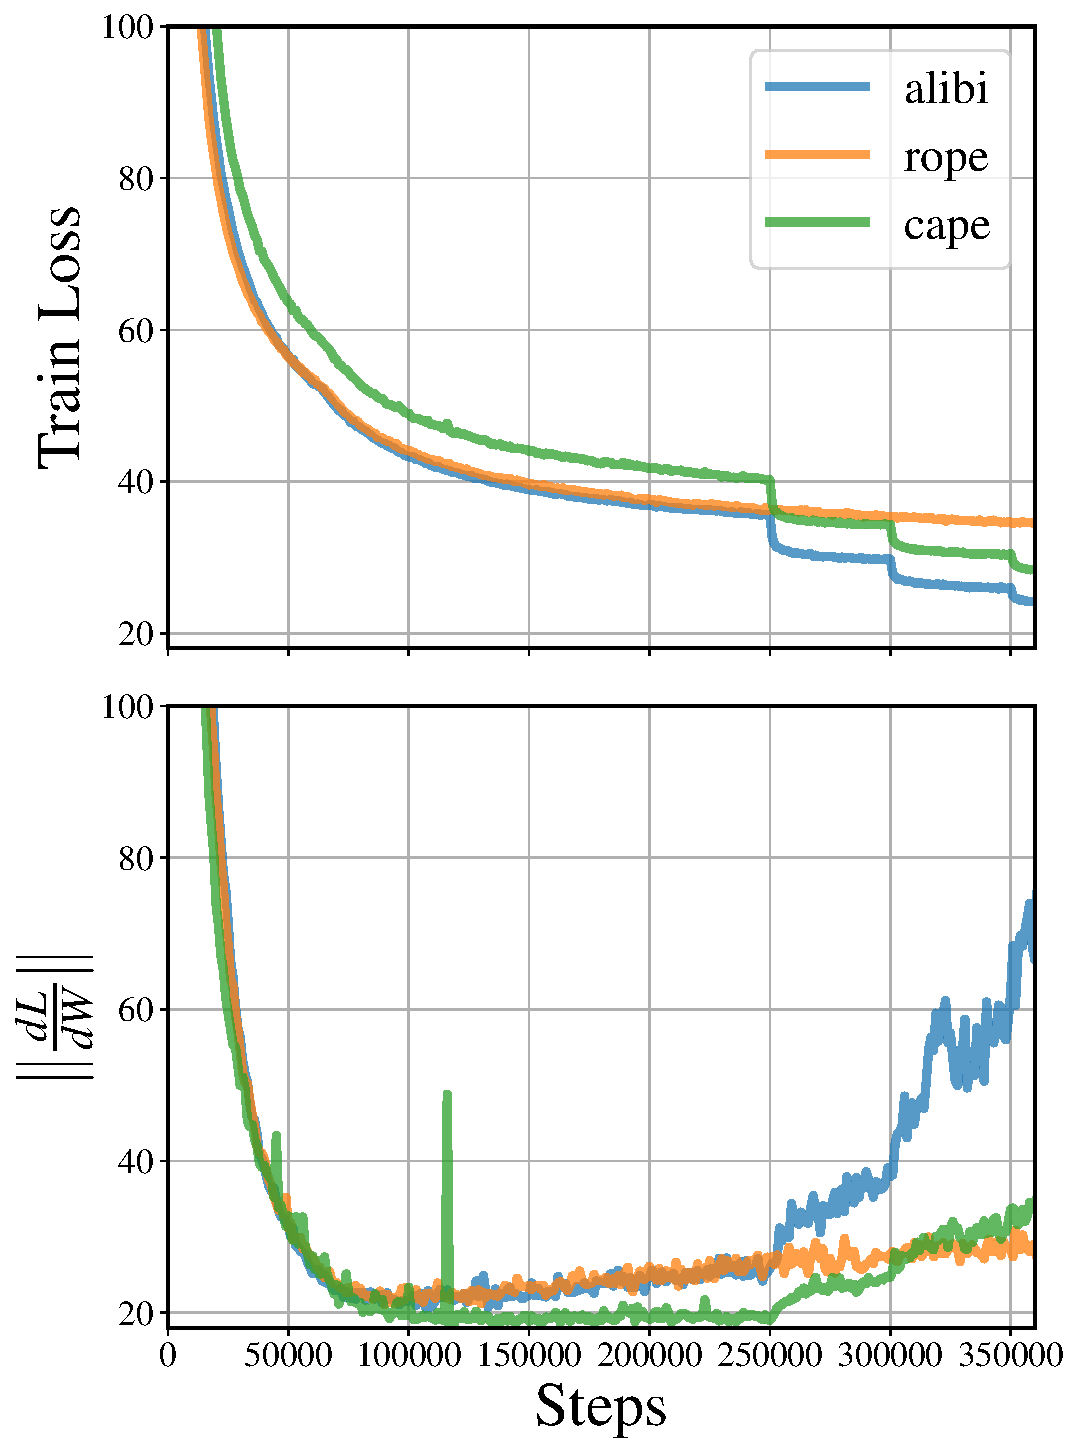
\includegraphics[width=0.6\linewidth]{figures/asr_appendix_pos_embed}
  \end{minipage}%
  \hfill
  \begin{minipage}{0.4\textwidth}
    \caption{ASR Transformer model (255M) training with pre-LayerNorm on LibriSpeech 960h with $\sigmoidattn$ (w/ bias term, $b=-\log n$, w/ QK norm, w/ LayerScale) and different positional embeddings CAPE, RoPE, ALiBi. The bias $b$ is able to stabilize $\sigmoidattn$ training: smooth training loss and only marginal rare spikes in gradient norms are observed.}    
    \label{fig:asr-logn}
  \end{minipage}  
\end{figure}

    

\subsubsection{Results and Ablations}
\label{sec:asr_appendix_ablations_and_results}
Initial investigation on post-LayerNorm and pre-LayerNorm transformers on both LibriSpeech 100h and 960h revealed that $\sigmoidattn$ without any bias is unstable resulting in huge and frequent gradient norm and training loss spikes throughout the training which in turn result in spikes of validation and test WER, see~\Cref{fig:asr-spikes}. Neither LayerScale nor QK norm were able to stabilize the training, though we did not observe any model divergence.

Further experiments with bias term in the $\sigmoidattn$ definition for post-LayerNorm transformers on LibriSpeech 100h reveal that training is now stable (only few marginal spikes in gradient norm occur, while train loss is smooth all the time). However, both LayerScale and QK norm restrict model capacity thus not matching $\softmaxattn$. Moreover, some combination of them is needed for the stable training, though w/o both of them we got the best performance for $\sigmoidattn$ (still behind $\softmaxattn$), see~\Cref{tab:asr-post-100h}.
We believe, further adaptation and deeper investigation is needed for $\sigmoidattn$ and post-LayerNorm, though recent advances in machine learning do not use post-LayerNorm models due to high training instability even for $\softmaxattn$.

Switching to pre-LayerNorm transformers and varying the depth of the models lead to stable training with $\sigmoidattn$ and bias term $b=-\log n$ with few (2-5 times) spikes in the gradient norm and smooth loss. In this case, $\sigmoidattn$ matches results for $\softmaxattn$ and they both generalize to TED-LIUM data similarly, see~\Cref{tab:asr-pre-100h}. If the bias term is removed, $\sigmoidattn$ can still match $\softmaxattn$ but large spikes in gradient norm and loss can occur.

Finally, we experiment with a conformer model, in \Cref{tab:asr-conformer}. Again, we found that bias term $b=-\log n$ stabilizes training. The learnable $b=-10$ works though we see significant gradient norm spikes while the train loss remains smooth. Besides,  $b=-\log n$ generalizes well to longer sequences while learnable $b=-10$ fails to do so with RoPE for conformer. Overall, $\sigmoidattn$ is able to match $\softmaxattn$ having stable training with  $b=-\log n$.

In experiments with different variants of bias term for $\sigmoidattn$, the bias $b=-\log n$ is found to be the most stable (only few marginal gradient norm spikes are observed with the train loss being smooth) and it provides similar performance as $\softmaxattn$ in most settings. 
The source of instability is coming from the larger attention output norms (80k for CAPE, 40k for RoPE and 20k for AliBi while being 200 for $\softmaxattn$). This happens due to high attention weight of every token which can be biased towards zero with a bias term in $\sigmoidattn$ definition.
Preliminary results to connect this to the local attention property needed at the beginning of the training for stable training failed, as local attention did not converge well at all (it is deactivated after some initial training).

To fully benefit from the improved throughput of \textsc{FlashSigmoid}, for the bias term $b=-\log n$ in $\sigmoidattn$, we experimented with configuration when the maximum audio duration in the minibatch is used as $n$ resulting into non-trainable bias scalar which changes between minibatches as we use dynamic batching. Comparison between the bias vector with per sample own duration normalization and the bias scalar as maximum duration in the minibatch is shown in ~\Cref{tab:asr-results-ext}: final model performance is similar and stability is same (only 2-3 minor spikes in CAPE for gradient norms are observed). Thus, per batch maximum audio duration can be used with $b=-\log n$ as the final configuration.

\begin{table}[t!]
\centering
\caption{Word error rate (\%) on LibriSpeech dev/test sets and TED-LIUM v3~\citep{hernandez2018ted} (``TED'', joint validation and test sets split according to  duration) for transformer (255M params) with either $\softmaxattn$ or $\sigmoidattn$ (LayerScale and QK norm are used with $b=-\log n$) trained on LibriSpeech 960h data (mean duration is 10-15s). Hyper-parameters are in~\cref{sec:asr_hps}.}
\label{tab:asr-results-ext}
\begin{center}
\begin{scriptsize}
\begin{sc}
\resizebox{\columnwidth}{!}{%
\begin{tabular}{lc|rrrr|rrrr}
\toprule
 attn & PE & dev-clean & test-clean & dev-other & test-other & ted 0-10s & ted 10-20s & ted 20-30s & ted 30s+  \\
\midrule 
softmax & \multirow{3}{*}{CAPE} & 2.2 & 2.3 & 5.6 & 5.7 & 12.4 & 10.5 & 11.9 & 9.1 \\
 sigmoid &  & 2.2 & 2.4 & 5.2 & 5.5 & 12.4 & 10.3 & 12.3 & 9.7 \\
 sigmoid, $b=-\log(\max_{batch} n)$ &  & 2.1 & 2.3 & 5.2 & 5.3 & 12.2 & 10.6 & 12.0 & 9.3 \\
\midrule
softmax & \multirow{3}{*}{RoPE} & 2.2 & 2.2 & 5.4 & 5.5 & 12.7 & 10.6 & 12.8 & 9.5 \\
 sigmoid &  & 2.0 & 2.3 & 5.2 & 5.4 & 12.3 & 10.1 & 12.3 & 8.6 \\
 sigmoid, $b=-\log(\max_{batch} n)$ & & 2.1 & 2.3 & 5.0 & 5.1  & 12.3 & 10.1 & 12.1 & 10.4 \\
\midrule
 softmax & \multirow{3}{*}{ALiBi} & 2.1 & 2.2 & 5.3 & 5.4 & 12.3 & 10.7 & 12.1 & 8.6 \\
 sigmoid &  & 2.1 & 2.3 & 5.0 & 5.1 & 12.3 & 10.5 & 12.6 & 9.1 \\
 sigmoid, $b=-\log(\max_{batch} n)$ &  & 2.0 & 2.3 & 5.2 & 5.2 & 12.3 & 10.5 & 11.9 & 10.2 \\
\bottomrule
\vspace{-0.4cm}
\end{tabular}
}
\end{sc}
\end{scriptsize}
\end{center}
\end{table}
